%% Volume I, Chapter 5: Limits and Continuity
\chapter{Limits and Continuity}
\label{ch:limits}

\abstract{An iterative method never reaches its answer: it produces approximations that, we hope, come ever closer to it. A discretisation is never exact: its error, we hope, disappears as the grid is refined. Both hopes are statements about limits, and so are almost all the guarantees of numerical analysis, from the convergence of an iteration to the claim that a small change in the data causes only a small change in the result. This chapter makes such statements precise. It defines limits of sequences and of functions, explains how limits are computed and why they exist, and proves the theorems on continuous functions on which root finding and optimisation rest.}

Calculus is the mathematics of change, and every one of its central notions, the derivative, the integral and the sum of an infinite series, is defined as a limit. This chapter, the first of Part~II, is about the limit itself. Most readers have computed many limits in a calculus course, usually by rules whose justification was left open. Here we revisit those rules and fill in the reasons: what it means for a sequence to converge, why the familiar limit laws hold, why certain limits exist even when nobody can write them down, and what continuity of a function buys.

Two earlier chapters prepared the ground. \Cref{ch:logic} introduced the definitions of the limit of a function (\cref{def:limit}) and of a sequence (\cref{def:sequence-limit}) as examples of statements with alternating quantifiers, and it proved that a sequence has at most one limit (\cref{thm:limit-unique}). \Cref{ch:numbers} described the real numbers as a complete ordered field and proved the first consequences of completeness: the Archimedean property (\cref{thm:archimedes}), the existence of roots (\cref{thm:roots}) and the convergence of bounded monotone sequences (\cref{thm:monotone}). We now use these tools in earnest. The reader will notice that completeness appears at every decisive point of the chapter: the limit laws hold in any ordered field, but every theorem asserting that some limit, root or maximum \emph{exists} rests on completeness and fails for the rational numbers.

The chapter has two halves. \Cref{sec:sequences,sec:limit-laws,sec:completeness} treat sequences: the definition of convergence and divergence, the rules for computing limits, and the theorems that guarantee convergence, among them the monotone convergence theorem, the nested interval theorem, the theorem of Bolzano and Weierstrass and the Cauchy criterion. \Cref{sec:function-limits,sec:continuity,sec:ivt,sec:evt,sec:uniform,sec:monotone-functions} treat functions: limits of functions, continuity, the intermediate value theorem with the bisection method that its proof contains, the extreme value theorem, uniform and Lipschitz continuity, and the continuity of inverse functions. As in the preceding chapters, this is a review: every result is stated precisely, the important ones are proved, and for the others the idea of the proof is given together with a reference. Volume~II returns to these topics in the generality of metric spaces.

\section{Sequences and Their Limits}
\label{sec:sequences}

A numerical method that improves an approximation step by step produces a sequence of numbers. The sequence is what we can compute; its limit, if there is one, is what we want. This section sets out the language for speaking about such sequences.

\subsection{Sequences}

A \term{sequence} of real numbers is a function $a\colon\mathbb N\to\mathbb R$, written with the argument as a subscript, $a_n$ instead of $a(n)$ (\cref{sec:functions}). We denote the whole sequence by $(a_n)_{n\in\mathbb N}$, or simply by $(a_n)$, and call $a_n$ its $n$th \term{term}. The brackets matter: $(a_n)$ is the sequence, $a_n$ a single number, and $\{a_n: n\in\mathbb N\}$ the set of the terms, which forgets their order and their repetitions. It is often convenient to start the indexing at some integer $n_0$ other than $0$, as in $(1/n)_{n\ge1}$; everything said below applies, with ``for all $n\ge n_0$'' in place of ``for all $n\in\mathbb N$''.

Sequences arise in several ways. Some are given by a formula for the $n$th term:
\begin{gather*}
\Bigl(\frac1n\Bigr)_{n\ge1}=\Bigl(1,\ \frac12,\ \frac13,\ \frac14,\ \ldots\Bigr),\\
\bigl((-1)^n\bigr)_{n\in\mathbb N}=(1,\ -1,\ 1,\ -1,\ \ldots),\qquad(r^n)_{n\in\mathbb N}=(1,\ r,\ r^2,\ \ldots).
\end{gather*}
Some are defined \term{recursively}, each term being computed from the previous ones. The rule
\begin{equation}
x_0\coloneqq1,\qquad x_{k+1}\coloneqq\frac12\Bigl(x_k+\frac2{x_k}\Bigr)\quad(k\in\mathbb N)
\label{eq:heron-def}
\end{equation}
produces $x_1=\frac32$, $x_2=\frac{17}{12}$, $x_3=\frac{577}{408}$, and so on; the recursion theorem (\cref{thm:recursion}), applied to the set $X=(0,\infty)$ and the function $g(x)=\frac12(x+2/x)$, which maps positive numbers to positive numbers, guarantees that such a rule defines exactly one sequence, and all its terms are positive, so that the division is always possible. Others are sums of a growing number of terms, such as the \term{partial sums} $s_n\coloneqq\sum_{k=1}^n1/k^2$ of an infinite series. Finally, every iterative algorithm defines a sequence: the approximations it produces after $1,2,3,\ldots$ steps.

A sequence can be pictured in two ways. One may mark the terms $a_0,a_1,a_2,\ldots$ as points on the real line, which shows where the terms lie but not their order, or one may plot the points $(n,a_n)$ in the plane, the graph of the function $n\mapsto a_n$. The second picture is usually more informative, and \cref{fig:eps-band} uses it.

\subsection{Convergence}

The definition of convergence was stated in \cref{def:sequence-limit}: a sequence $(a_n)$ \term{converges} to the real number $L$, written $a_n\to L$, if
\begin{equation}
\forall\varepsilon>0,\ \exists N\in\mathbb N,\ \forall n\ge N:\quad|a_n-L|<\varepsilon .
\label{eq:seq-limit}
\end{equation}
The number $L$ is a \term{limit} of the sequence. The inequality $|a_n-L|<\varepsilon$ says that $a_n$ lies in the open interval $(L-\varepsilon,L+\varepsilon)$, a band of half-width $\varepsilon$ around $L$. The definition therefore says: however narrow the band, from some index on all terms lie inside it. Finitely many terms may lie outside, but only finitely many, and which ones depends on the width of the band. \Cref{fig:eps-band} shows the situation for one band.

\begin{figure}
\sdfloat{%
\begin{tikzpicture}
\begin{axis}[sdplot, width=0.66\textwidth, height=0.42\textwidth, xmin=-1, xmax=31, ymin=0, ymax=2.6,
  xtick={0,7,20,30}, xticklabels={0,$N=7$,20,30},
  ytick={0,0.8,1,1.2,2}, yticklabels={0,$L-\varepsilon$,$L$,$L+\varepsilon$,2},
  xlabel={$n$}, ylabel={$a_n$}]
\fill[sdfill] (axis cs:-1,0.8) rectangle (axis cs:31,1.2);
\draw[black!55, dashed, line width=0.4pt] (axis cs:7,0) -- (axis cs:7,2.6);
\addplot[black, only marks, mark=o, mark size=1.4pt] coordinates {(0,2.5) (1,0.25) (2,1.5) (3,0.625) (4,1.3) (5,0.75) (6,1.21429)};
\addplot[black, only marks, mark=*, mark size=1.3pt] coordinates {(7,0.8125) (8,1.16667) (9,0.85) (10,1.13636) (11,0.875) (12,1.11538) (13,0.89286) (14,1.1) (15,0.90625) (16,1.08824) (17,0.91667) (18,1.07895) (19,0.925) (20,1.07143) (21,0.93182) (22,1.06522) (23,0.9375) (24,1.06) (25,0.94231) (26,1.05556) (27,0.94643) (28,1.05172) (29,0.95) (30,1.04839)};
\end{axis}
\end{tikzpicture}}{The sequence $a_n=1+(-1)^n\cdot1.5/(n+1)$, which converges to $L=1$. For $\varepsilon=0.2$ the band $(L-\varepsilon,L+\varepsilon)$ is shaded. The terms with $n\ge N=7$ (filled) all lie inside it; of the earlier terms (open circles), all lie outside. A narrower band would require a larger $N$.\label{fig:eps-band}}
\end{figure}

For the sequence of the figure, $|a_n-1|=1.5/(n+1)$, and this is less than $\varepsilon$ exactly when $n+1>1.5/\varepsilon$. For $\varepsilon=0.2$ the first index that works is $N=7$; for $\varepsilon=0.01$ it is $N=150$. In the language of the game of \cref{sec:quantifiers}, the sceptic names a tolerance $\varepsilon$, the prover answers with an index $N$, and the prover must win for every tolerance. The answer may depend on $\varepsilon$, and it usually must. It need not be the smallest index that works: if $N$ works, so does every larger index, and in proofs one is free to choose generously.

A statement $P(n)$ about the index $n$ is said to hold \term{eventually}, or \term{for all sufficiently large $n$}, if there is an $N$ such that $P(n)$ holds for all $n\ge N$. In this language, $a_n\to L$ means that for every $\varepsilon>0$, eventually $|a_n-L|<\varepsilon$. If two statements each hold eventually, so does their conjunction: if the first holds from $N_1$ on and the second from $N_2$ on, both hold from $\max(N_1,N_2)$ on. This simple observation is used in almost every proof of this section.

The definition can be varied in harmless ways, and it is useful to know which variations are harmless. The proofs below often end with an estimate such as $|a_n-L|<2\varepsilon$ or $|a_n-L|\le\varepsilon$ instead of $|a_n-L|<\varepsilon$.

\begin{proposition}
\label{prop:limit-variants}
Let $(a_n)$ be a sequence, $L$ a real number and $C>0$ a constant. The following statements are equivalent.
\begin{enumerate}
\item $a_n\to L$.
\item For every $\varepsilon>0$ there is $N$ such that $|a_n-L|\le\varepsilon$ for all $n\ge N$.
\item For every $\varepsilon>0$ there is $N$ such that $|a_n-L|<C\varepsilon$ for all $n\ge N$.
\end{enumerate}
\end{proposition}

\begin{proof}
(i) implies (ii), because $|a_n-L|<\varepsilon$ implies $|a_n-L|\le\varepsilon$. (ii) implies (i): given $\varepsilon>0$, apply (ii) to $\varepsilon/2$; then $|a_n-L|\le\varepsilon/2<\varepsilon$ from some $N$ on. (i) implies (iii): given $\varepsilon>0$, apply (i) to the positive number $C\varepsilon$. (iii) implies (i): given $\varepsilon>0$, apply (iii) to $\varepsilon/C$.
\end{proof}

The next proposition records three facts that are used constantly. Part (i) reduces every question of convergence to a question of convergence to zero, and part (iii) says that the beginning of a sequence is irrelevant to its limit: convergence is a property of the tail.

\begin{proposition}
\label{prop:seq-basic}
Let $(a_n)$ be a sequence and $L$ a real number.
\begin{enumerate}
\item $a_n\to L$ if and only if $a_n-L\to0$, and if and only if $|a_n-L|\to0$.
\item If $a_n\to L$, then $|a_n|\to|L|$.
\item Let $(b_n)$ be a sequence and $p\in\mathbb N$ such that $b_n=a_{n+p}$ for all sufficiently large $n$. Then $a_n\to L$ if and only if $b_n\to L$. In particular, changing finitely many terms of a sequence does not change whether it converges, or its limit.
\end{enumerate}
\end{proposition}

\begin{proof}
(i) All three statements say that for every $\varepsilon>0$, eventually $|a_n-L|<\varepsilon$, since $|(a_n-L)-0|=\bigl||a_n-L|-0\bigr|=|a_n-L|$.

(ii) By the reverse triangle inequality (\cref{cor:reverse-triangle}), $\bigl||a_n|-|L|\bigr|\le|a_n-L|$, so $|a_n|$ lies within $\varepsilon$ of $|L|$ whenever $a_n$ lies within $\varepsilon$ of $L$.

(iii) Suppose $b_n=a_{n+p}$ for all $n\ge N_0$. If $|a_n-L|<\varepsilon$ for all $n\ge N$, then $|b_n-L|=|a_{n+p}-L|<\varepsilon$ for all $n\ge\max(N,N_0)$, since then $n+p\ge N$. Conversely, if $|b_n-L|<\varepsilon$ for all $n\ge N$, then $|a_m-L|=|b_{m-p}-L|<\varepsilon$ for all $m\ge\max(N,N_0)+p$. If $(b_n)$ arises from $(a_n)$ by changing finitely many terms, the statement applies with $p=0$.
\end{proof}

The converse of (ii) fails: $|(-1)^n|\to1$, but, as we show next, $(-1)^n$ does not converge at all. It holds when $L=0$, by (i).

\emph{Examples.} The following computations show the definition at work; each exhibits, for a given $\varepsilon$, an index $N$ that wins the game.

The sequence $(1/n)_{n\ge1}$ converges to $0$. Let $\varepsilon>0$. By the Archimedean property, in the form of \cref{cor:archimedes}\,(i), there is an integer $N\ge1$ with $1/N<\varepsilon$, and then $|1/n-0|=1/n\le1/N<\varepsilon$ for all $n\ge N$. This limit, together with completeness, is behind almost every other limit in this chapter.

The sequence $a_n=(n+1)/(2n+3)$ converges to $\frac12$. As in \cref{sec:quantifiers}, we first work out how large $n$ must be. Bringing the difference to a common denominator,
\[
\Bigl|\frac{n+1}{2n+3}-\frac12\Bigr|=\Bigl|\frac{2(n+1)-(2n+3)}{2(2n+3)}\Bigr|=\frac1{4n+6}<\frac1n\qquad(n\ge1).
\]
So given $\varepsilon>0$ it suffices to choose an integer $N\ge1$ with $1/N<\varepsilon$, as before; then $|a_n-\frac12|<1/n\le1/N<\varepsilon$ for all $n\ge N$. The estimate $1/(4n+6)<1/n$ is wasteful, but a proof needs some $N$ that works, not the best one.

The sequence $\bigl((-1)^n\bigr)$ converges to no real number. Suppose it converged to $L$. With $\varepsilon\coloneqq1$ there would be an $N$ with $|(-1)^n-L|<1$ for all $n\ge N$, in particular for $n=N$ and $n=N+1$. One of the two terms is $1$ and the other $-1$, so the triangle inequality would give
\[
2=|1-(-1)|\le|1-L|+|L-(-1)|<1+1=2,
\]
which is impossible. The argument is the one that showed in \cref{prop:step-no-limit} that the step function has no limit at $0$: two values that are far apart cannot both lie close to a single number.

By \cref{thm:limit-unique}, a sequence converges to at most one number. If it converges to $L$, we call $L$ \emph{the} limit and write
\[
\lim_{n\to\infty}a_n=L .
\]
A sequence is \term{convergent} if it converges to some real number and \term{divergent} otherwise. The notation $\lim_{n\to\infty}a_n$ may be used only once the limit is known to exist; an equation such as $\lim_{n\to\infty}(-1)^n=L$ is not false but meaningless. The symbol $\infty$ in it does not denote a number: ``$n\to\infty$'' is shorthand for the phrase ``as $n$ grows without bound'' and refers to the form of the definition, in which $n$ is required to be large.

\subsection{Bounded Sequences}

\begin{definition}[Bounded sequence]
\label{def:bounded-seq}
A sequence $(a_n)$ is \term{bounded above} if there is a real number $C$ with $a_n\le C$ for all $n$, \term{bounded below} if there is $c$ with $a_n\ge c$ for all $n$, and \term{bounded} if it is both, that is, if there is $C$ with $|a_n|\le C$ for all $n$.
\end{definition}

\begin{proposition}
\label{prop:convergent-bounded}
Every convergent sequence is bounded.
\end{proposition}

\begin{proof}
Let $a_n\to L$. With $\varepsilon\coloneqq1$ there is $N$ such that $|a_n-L|<1$ for all $n\ge N$, and then $|a_n|\le|a_n-L|+|L|<|L|+1$ by the triangle inequality. Only the finitely many terms $a_0,\ldots,a_{N-1}$ remain, and
\[
C\coloneqq\max\bigl(|a_0|,\ |a_1|,\ \ldots,\ |a_{N-1}|,\ |L|+1\bigr)
\]
satisfies $|a_n|\le C$ for every $n$.
\end{proof}

The proof shows a pattern that recurs: a property that the tail has because it is close to $L$, and the finitely many terms before the tail have because there are finitely many of them. The converse of the proposition is false, as the bounded divergent sequence $\bigl((-1)^n\bigr)$ shows. In contrapositive form the proposition is a test for divergence: an unbounded sequence diverges. For instance, $(n^2)$ is unbounded, by the Archimedean property, and therefore divergent.

\subsection{Divergence to Infinity}

An unbounded sequence diverges, but it may do so in an orderly way. The terms of $(n^2)$ do not approach any number; they grow beyond every bound and stay there. This behaviour deserves a name of its own.

\begin{definition}[Divergence to infinity]
\label{def:diverge-infinity}
A sequence $(a_n)$ \term{diverges to infinity}, written $a_n\to\infty$ or $\lim_{n\to\infty}a_n=\infty$, if
\[
\forall M\in\mathbb R,\ \exists N\in\mathbb N,\ \forall n\ge N:\quad a_n>M .
\]
It \term{diverges to minus infinity}, written $a_n\to-\infty$, if $-a_n\to\infty$, that is, if for every $M$, eventually $a_n<M$.
\end{definition}

The roles are the same as in \eqref{eq:seq-limit}: the sceptic names a level $M$, as high as desired, and the prover must find an index beyond which all terms exceed it. For $a_n=n^2$, given $M$ choose by the Archimedean property an integer $N\ge1$ with $N>M$; then $n^2\ge n\ge N>M$ for $n\ge N$. Similarly $2^n\to\infty$, because $2^n=(1+1)^n\ge1+n$ by Bernoulli's inequality (\cref{thm:bernoulli}), and $-\sqrt n\to-\infty$, because $\sqrt n>|M|$ as soon as $n>M^2$.

Two remarks prevent misunderstandings. First, a sequence that diverges to infinity is still divergent. The words ``convergent'' and ``limit'' without qualification always refer to a real number, and the symbols $\infty$ and $-\infty$ are not real numbers; they occur only in the phrases ``$a_n\to\infty$'' and ``$\lim a_n=\infty$'', which abbreviate the definition above. Second, an unbounded sequence need not diverge to infinity. The sequence that equals $n$ for even $n$ and $0$ for odd $n$ is unbounded, but it returns to $0$ infinitely often, so it does not eventually exceed $M=1$. The same holds for $\bigl((-1)^nn\bigr)$, which is unbounded in both directions.

\section{Limit Laws for Sequences}
\label{sec:limit-laws}

Proving every limit from the definition would be tedious. In practice one proves a handful of basic limits from the definition and derives the rest from them with a few general rules. This section establishes the rules: limits respect the arithmetic operations and the order, and a sequence trapped between two sequences with the same limit has that limit too~\cite{spivak2008calculus,abbott2015}. It ends with a list of standard limits and a first encounter with the number $e$.

\subsection{Arithmetic of Limits}

\begin{theorem}[Limit laws]
\label{thm:limit-laws}
Let $a_n\to L$ and $b_n\to M$, and let $c$ be a real number. Then:
\begin{enumerate}
\item $a_n+b_n\to L+M$ and $a_n-b_n\to L-M$;
\item $ca_n\to cL$;
\item $a_nb_n\to LM$;
\item if $M\ne0$, then $b_n\ne0$ for all sufficiently large $n$, and $a_n/b_n\to L/M$.
\end{enumerate}
\end{theorem}

\begin{proof}
(i) Let $\varepsilon>0$. Eventually $|a_n-L|<\varepsilon/2$, and eventually $|b_n-M|<\varepsilon/2$; so eventually both hold, and then
\[
|(a_n+b_n)-(L+M)|\le|a_n-L|+|b_n-M|<\frac\varepsilon2+\frac\varepsilon2=\varepsilon .
\]
The difference is treated in the same way, since $|(a_n-b_n)-(L-M)|\le|a_n-L|+|b_n-M|$.

(iii) The idea is to split the change from $LM$ to $a_nb_n$ into a change of one factor at a time:
\[
a_nb_n-LM=a_n(b_n-M)+M(a_n-L).
\]
By \cref{prop:convergent-bounded} there is $C>0$ with $|a_n|\le C$ for all $n$. Let $\varepsilon>0$. Eventually $|b_n-M|<\varepsilon/(2C)$ and $|a_n-L|<\varepsilon/(2|M|+1)$, and then
\[
|a_nb_n-LM|\le C|b_n-M|+|M|\,|a_n-L|<\frac\varepsilon2+\frac{|M|\varepsilon}{2|M|+1}<\varepsilon .
\]
(The denominator $2|M|+1$ instead of $2|M|$ avoids a division by zero when $M=0$.)

(ii) This is (iii) with the constant sequence $b_n=c$, which converges to $c$.

(iv) By (iii) it suffices to show that $1/b_n\to1/M$. By \cref{prop:seq-basic}\,(ii), $|b_n|\to|M|>0$, so with $\varepsilon\coloneqq|M|/2$ there is $N$ with $|b_n|>|M|/2$ for all $n\ge N$; in particular $b_n\ne0$ for these $n$. For $n\ge N$,
\[
\Bigl|\frac1{b_n}-\frac1M\Bigr|=\frac{|M-b_n|}{|b_n|\,|M|}\le\frac{2}{|M|^2}\,|b_n-M| .
\]
Given $\varepsilon>0$, eventually $|b_n-M|<|M|^2\varepsilon/2$, and then the right side is less than $\varepsilon$.
\end{proof}

The proof of (iii) contains the idea of most error estimates for products: the error in a product of approximations is bounded by the size of one factor times the error of the other, plus the size of the second factor times the error of the first. In (iv), the quotient $a_n/b_n$ may be undefined for finitely many $n$; by \cref{prop:seq-basic}\,(iii) this does not matter, and we regard $(a_n/b_n)$ as a sequence that starts at the first index after which $b_n$ never vanishes.

By induction, (iii) gives $a_n^k\to L^k$ for every $k\in\mathbb N$, and together with (i) and (ii) it gives $p(a_n)\to p(L)$ for every polynomial $p$. Quotients of polynomials in $n$ are handled by dividing numerator and denominator by the highest power of $n$ that occurs in the denominator. For example,
\[
\frac{3n^2+n}{n^2-5}=\frac{3+1/n}{1-5/n^2}\to\frac{3+0}{1-0}=3 ,
\]
by (i), (ii), (iii) and (iv) and the limit $1/n\to0$, which gives $1/n^2=(1/n)(1/n)\to0$. The same computation shows that the quotient of two polynomials in $n$ of the same degree tends to the quotient of their leading coefficients, and that the quotient tends to $0$ when the numerator has the smaller degree.

The hypotheses of the theorem are that $(a_n)$ and $(b_n)$ converge, and they cannot be dropped. With $a_n=(-1)^n$ and $b_n=-(-1)^n$ the sum $a_n+b_n=0$ converges, although neither summand does. So the theorem may be used to compute the limit of a sum from the limits of its terms, but not to conclude anything about the terms from the sum.

\subsection{Limits and Order}

\begin{proposition}
\label{prop:limit-order}
Let $a_n\to L$ and $b_n\to M$.
\begin{enumerate}
\item If $L<M$, then $a_n<b_n$ for all sufficiently large $n$. In particular, if $L<c$ for a real number $c$, then eventually $a_n<c$, and if $L>0$, then eventually $a_n>0$.
\item If $a_n\le b_n$ for all sufficiently large $n$, then $L\le M$. In particular, if $c\le a_n\le d$ for all sufficiently large $n$, then $c\le L\le d$.
\end{enumerate}
\end{proposition}

\begin{proof}
(i) Let $\varepsilon\coloneqq(M-L)/2>0$. Eventually $a_n<L+\varepsilon$ and $b_n>M-\varepsilon$, and $L+\varepsilon=M-\varepsilon$ is the midpoint of $L$ and $M$; so eventually $a_n<\frac{L+M}2<b_n$. The special cases follow by comparing $(a_n)$ with the constant sequence $(c)$, and the constant sequence $(0)$ with $(a_n)$.

(ii) If $L>M$, then (i), with the roles of the two sequences exchanged, would give $b_n<a_n$ for all sufficiently large $n$, contradicting the hypothesis, because the two conditions ``eventually'' would hold simultaneously from some index on. So $L\le M$. The special case follows with constant sequences.
\end{proof}

Strict inequalities between the terms do not survive in the limit: $1/n>0$ for every $n\ge1$, but $\lim1/n=0$. The terms of a sequence in the open interval $(0,1)$ may converge to $0$ or to $1$, which are not in the interval, whereas by (ii) the limit of a convergent sequence in a closed interval $[c,d]$ lies in $[c,d]$. This difference between open and closed intervals returns in \cref{sec:evt}, where it decides whether a function attains its maximum.

The next theorem is the most frequently used tool for proving that a limit exists. It is known as the \term{squeeze theorem}, or the sandwich theorem.

\begin{theorem}[Squeeze theorem]
\label{thm:squeeze}
Let $(a_n)$, $(b_n)$ and $(c_n)$ be sequences with $a_n\le c_n\le b_n$ for all sufficiently large $n$. If $a_n\to L$ and $b_n\to L$, then $c_n\to L$.
\end{theorem}

\begin{proof}
Let $\varepsilon>0$. Eventually all three of $a_n\le c_n\le b_n$, $a_n>L-\varepsilon$ and $b_n<L+\varepsilon$ hold, and then $L-\varepsilon<a_n\le c_n\le b_n<L+\varepsilon$, that is, $|c_n-L|<\varepsilon$.
\end{proof}

Unlike \cref{prop:limit-order}\,(ii), the theorem does not assume that $(c_n)$ converges; it proves it. The most common application is to error bounds.

\begin{corollary}
\label{cor:squeeze-zero}
If $|a_n-L|\le e_n$ for all sufficiently large $n$ and $e_n\to0$, then $a_n\to L$.
\end{corollary}

\begin{proof}
Apply \cref{thm:squeeze} to $0\le|a_n-L|\le e_n$ and use \cref{prop:seq-basic}\,(i).
\end{proof}

This is the form in which convergence is proved for numerical methods. One rarely knows the error $|a_n-L|$ of the $n$th approximation, since $L$ is the unknown, but one can often prove a bound $e_n$ for it that is known to tend to zero. The bisection method of \cref{sec:ivt}, for instance, comes with the bound $e_k=(b-a)/2^{k+1}$ after $k$ steps. As examples of the corollary, $(-1)^n/n\to0$ because $|(-1)^n/n|=1/n\to0$, and $(\sin n)/n\to0$ because $|\sin n|\le1$ by \cref{asm:trig}\,(i).

\subsection{Infinite Limits}

The arithmetic of divergence to infinity follows the intuition that a huge number plus a moderate one is huge, and that the reciprocal of a huge number is tiny.

\begin{proposition}
\label{prop:infinite-laws}
Let $(a_n)$ and $(b_n)$ be sequences.
\begin{enumerate}
\item If $a_n\to\infty$ and $(b_n)$ is bounded below, then $a_n+b_n\to\infty$.
\item If $a_n\to\infty$ and there is $c>0$ with $b_n\ge c$ for all sufficiently large $n$, then $a_nb_n\to\infty$.
\item If $a_n\to\infty$ and $a_n\le b_n$ for all sufficiently large $n$, then $b_n\to\infty$.
\item If $|a_n|\to\infty$, then $a_n\ne0$ eventually and $1/a_n\to0$.
\item If $a_n\to0$ and $a_n>0$ for all sufficiently large $n$, then $1/a_n\to\infty$.
\end{enumerate}
\end{proposition}

\begin{proof}
(i) Let $b_n\ge c$ for all $n$, and let $M$ be given. Eventually $a_n>M-c$, and then $a_n+b_n>M$. (ii) Given $M$, eventually $a_n>\max(M,0)/c$ and $b_n\ge c$, so $a_nb_n>\max(M,0)\ge M$. (iii) Eventually $b_n\ge a_n>M$. (iv) Given $\varepsilon>0$, eventually $|a_n|>1/\varepsilon$, so that $a_n\ne0$ and $|1/a_n|<\varepsilon$. (v) Given $M$, put $\varepsilon\coloneqq1/\max(M,1)$; eventually $0<a_n<\varepsilon$, and then $1/a_n>\max(M,1)\ge M$.
\end{proof}

No such rules exist for the \term{indeterminate forms} $\infty-\infty$, $0\cdot\infty$, $\infty/\infty$ and $0/0$, because the outcome depends on how fast the two parts grow or shrink. With $a_n=n$ the sequences $a_n-b_n$ for $b_n=n$, $b_n=n-1$ and $b_n=\sqrt n$ tend to $0$, to $1$ and to $\infty$ respectively, although $a_n$ and $b_n$ diverge to infinity in all three cases; and $(1/n)\cdot n\to1$ while $(1/n^2)\cdot n\to0$. An indeterminate form signals that the limit must be found by other means, typically by rewriting the expression as we did for quotients of polynomials.

\subsection{Standard Limits}

The following limits occur so often that they are worth knowing by heart. They describe how powers, exponentials and factorials compare as $n$ grows; several of them, with similar proofs, are collected in Rudin's text~\cite{rudin1976}.

\begin{theorem}[Standard limits]
\label{thm:standard-limits}
\leavevmode
\begin{enumerate}
\item For every rational number $p>0$, $1/n^p\to0$.
\item For a real number $r$: if $|r|<1$, then $r^n\to0$; if $r=1$, then $r^n\to1$; if $r>1$, then $r^n\to\infty$; and if $r\le-1$, then $(r^n)$ diverges and does not diverge to $\infty$ or to $-\infty$.
\item For every real number $a>0$, $a^{1/n}\to1$.
\item $n^{1/n}\to1$.
\item For every $k\in\mathbb N$ and every real $r$ with $|r|<1$, $n^kr^n\to0$.
\item For every real number $r$, $r^n/n!\to0$.
\item $n!/n^n\to0$.
\end{enumerate}
\end{theorem}

\begin{proof}
(i) Write $p=s/t$ with integers $s,t\ge1$. For $n\ge1$ we have $n^{1/t}\ge1$, so $n^p=(n^{1/t})^s\ge n^{1/t}$. Given $\varepsilon>0$, choose an integer $N>\varepsilon^{-t}$. For $n\ge N$, \cref{prop:ineq-rules}\,(iii) gives $n^{1/t}\ge N^{1/t}>(\varepsilon^{-t})^{1/t}=1/\varepsilon$, so $0<1/n^p\le1/n^{1/t}<\varepsilon$.

(ii) If $|r|<1$, then $|r^n|=|r|^n\to0$ by \eqref{eq:rn-zero}, and $r^n\to0$ by \cref{prop:seq-basic}\,(i). The case $r=1$ is trivial. If $r>1$, write $r=1+h$ with $h>0$; Bernoulli's inequality gives $r^n\ge1+nh$, and $1+nh\to\infty$, so $r^n\to\infty$ by \cref{prop:infinite-laws}\,(iii). If $r\le-1$, the terms alternate in sign, so $(r^n)$ cannot eventually exceed $0$ or eventually stay below it, and $|r^n-r^{n+1}|=|r|^n\,|1-r|\ge2$ for all $n$, so two consecutive terms are never within distance $1$ of a common number $L$, and the argument used above for $(-1)^n$ excludes convergence.

(iii) Suppose first $a\ge1$. Then $a^{1/n}\ge1$; write $a^{1/n}=1+h_n$ with $h_n\ge0$. By Bernoulli's inequality, $a=(1+h_n)^n\ge1+nh_n$, so $0\le h_n\le(a-1)/n$, and $h_n\to0$ by the squeeze theorem. If $0<a<1$, then $1/a>1$ and $a^{1/n}=1/(1/a)^{1/n}\to1/1=1$ by the first case and \cref{thm:limit-laws}\,(iv).

(iv) For $n\ge2$, write $n^{1/n}=1+h_n$ with $h_n\ge0$. By the binomial theorem (\cref{thm:binomial}), all of whose terms are nonnegative here,
\[
n=(1+h_n)^n\ge1+\binom n2h_n^2=1+\frac{n(n-1)}2h_n^2 ,
\]
so $h_n^2\le2/n$ and $0\le h_n\le\sqrt2\,n^{-1/2}$. By (i) with $p=\frac12$ and the squeeze theorem, $h_n\to0$.

(v) For $r=0$ there is nothing to prove. Otherwise $1/|r|=1+h$ with $h>0$. For $n\ge2k+2$, the binomial theorem gives
\[
(1+h)^n\ge\binom n{k+1}h^{k+1}=\frac{n(n-1)\cdots(n-k)}{(k+1)!}h^{k+1}\ge\frac{(n/2)^{k+1}}{(k+1)!}h^{k+1} ,
\]
because each of the $k+1$ factors $n-j$ with $0\le j\le k$ is at least $n/2$. Hence
\[
|n^kr^n|=\frac{n^k}{(1+h)^n}\le\frac{2^{k+1}(k+1)!}{h^{k+1}}\cdot\frac1n ,
\]
a constant times $1/n$, and $n^kr^n\to0$ by \cref{cor:squeeze-zero}.

(vi) Choose an integer $K\ge1$ with $K\ge2|r|$. For $n>K$,
\[
\frac{|r|^n}{n!}=\frac{|r|^K}{K!}\prod_{j=K+1}^{n}\frac{|r|}{j}\le\frac{|r|^K}{K!}\Bigl(\frac12\Bigr)^{n-K},
\]
because each factor $|r|/j$ is at most $|r|/K\le\frac12$. The right side is a constant times $2^{-n}$, which tends to $0$ by (ii).

(vii) For $n\ge1$, $n!/n^n=\frac1n\cdot\frac2n\cdots\frac nn\le\frac1n$, since every factor after the first is at most $1$.
\end{proof}

Parts (v), (vi) and (vii) establish a hierarchy: every power $n^k$ is eventually negligible compared with every exponential $s^n$ with $s>1$ (take $r=1/s$ in (v)), every exponential is negligible compared with $n!$, and $n!$ is negligible compared with $n^n$. \Cref{tab:growth} shows how quickly the gaps open. The hierarchy is the reason why an algorithm whose running time grows like a power of the input size is called efficient and one that grows exponentially is not (Volume~IV): for $n=50$, an algorithm with $n^3$ steps takes $125\,000$ steps, and one with $2^n$ steps takes more than a million billion. The growth of $n!$ itself is described precisely by Stirling's formula in Chapter~8.

\begin{table}
\sdfloat{%
\begin{sdtable}{colspec={rrrrr}, row{1}={font=\small\bfseries}}
\toprule
$n$ & $n^3$ & $2^n$ & $n!$ & $n^n$ \\
\midrule
10 & $1\,000$ & $1\,024$ & $3.6\times10^{6}$ & $10^{10}$ \\
20 & $8\,000$ & $1\,048\,576$ & $2.4\times10^{18}$ & $1.0\times10^{26}$ \\
50 & $125\,000$ & $1.1\times10^{15}$ & $3.0\times10^{64}$ & $8.9\times10^{84}$ \\
100 & $1\,000\,000$ & $1.3\times10^{30}$ & $9.3\times10^{157}$ & $10^{200}$ \\
\bottomrule
\end{sdtable}}{Powers, exponentials and factorials; numbers written with a power of ten are rounded to two significant digits. Each column is eventually negligible compared with the next one (\cref{thm:standard-limits}).\label{tab:growth}}
\end{table}

\subsection{A First Look at the Number \texorpdfstring{$e$}{e}}

Late in the seventeenth century Jacob Bernoulli considered a problem of compound interest~\cite{maor1994}. A sum of money earns interest at the rate of $100$ per cent a year. If the interest is paid once, at the end of the year, the capital doubles. If it is paid twice, at $50$ per cent each half year, and the interest of the first half year earns interest in the second, the capital is multiplied by $(1+\frac12)^2=2.25$. With $n$ payments of $1/n$ each, the factor is
\[
a_n\coloneqq\Bigl(1+\frac1n\Bigr)^n .
\]
Does the factor grow without bound as the interest is paid more and more often? \Cref{tab:compound} suggests that it does not: the values increase, but ever more slowly, and they appear to approach a number slightly larger than $2.718$.

\begin{table}
\sdfloat{%
\begin{sdtable}{colspec={rll}, row{1}={font=\small\bfseries}}
\toprule
$n$ & $(1+1/n)^n$ & $(1+1/n)^{n+1}$ \\
\midrule
1 & 2 & 4 \\
2 & 2.25 & 3.375 \\
10 & 2.593742\ldots & 2.853116\ldots \\
100 & 2.704813\ldots & 2.731861\ldots \\
1\,000 & 2.716923\ldots & 2.719640\ldots \\
10\,000 & 2.718145\ldots & 2.718417\ldots \\
1\,000\,000 & 2.718280\ldots & 2.718283\ldots \\
\bottomrule
\end{sdtable}}{Compound interest. With $n$ payments of interest at the rate $1/n$, a capital is multiplied by $(1+1/n)^n$. The left column increases and the right column decreases; both approach $e=2.718281\ldots$ (\cref{thm:e}).\label{tab:compound}}
\end{table}

None of the limit laws applies here. The base $1+1/n$ tends to $1$, which suggests the limit $1$, while the exponent tends to infinity, which suggests that small excesses over $1$ accumulate without bound; the expression is an indeterminate form of the type $1^\infty$. Nor can we guess the limit, if there is one, and then verify it with the definition: the number in question has no simpler description. What is needed is a theorem that guarantees the existence of a limit without naming it, and this is the subject of the next section. There we shall see that the sequences in both columns of the table converge, to the same number $e$.

\section{Monotone Sequences and Completeness}
\label{sec:completeness}

The limit laws compute limits from known limits; they never produce a limit out of nothing. To show that $(1+1/n)^n$ converges, we need a principle that guarantees the existence of a limit from properties of the terms alone. Such principles cannot be proved from the axioms of an ordered field, because they fail in $\mathbb Q$. The recursive sequence \eqref{eq:heron-def} consists of rational numbers, and we shall see that it converges to $\sqrt2$, which is irrational (\cref{thm:sqrt2}); regarded as a sequence in $\mathbb Q$, it has no limit. Every existence theorem of this section therefore rests on the completeness axiom of \cref{def:complete}. The four general principles proved here, the monotone convergence theorem, the nested interval theorem, the theorem of Bolzano and Weierstrass and the Cauchy criterion, are each equivalent to that axiom in the presence of the Archimedean property, as the note at the end of the section explains.

\subsection{Monotone Sequences}

Recall from \cref{sec:reals} that a sequence $(a_n)$ is \term{increasing} if $a_n\le a_{n+1}$ for all $n$ and \term{decreasing} if $a_n\ge a_{n+1}$ for all $n$. We call it \term{strictly increasing} or \term{strictly decreasing} if the inequalities are strict, and \term{monotone} if it is increasing or decreasing. The monotone convergence theorem, \cref{thm:monotone}, says that an increasing sequence that is bounded above converges to the supremum of its terms, and that a decreasing sequence that is bounded below converges to the infimum of its terms. The proof was short: for every $\varepsilon>0$ some term exceeds $\sup_na_n-\varepsilon$, by the approximation property of the supremum (\cref{lem:sup-approx}), and all later terms are at least as large and still at most the supremum. Completeness enters through the existence of the supremum. Combined with \cref{prop:convergent-bounded}, the theorem gives a complete description of monotone sequences.

\begin{corollary}
\label{cor:monotone-dichotomy}
A monotone sequence converges if and only if it is bounded. An increasing sequence that is not bounded above diverges to $\infty$, and a decreasing sequence that is not bounded below diverges to $-\infty$.
\end{corollary}

\begin{proof}
A convergent sequence is bounded by \cref{prop:convergent-bounded}. An increasing sequence is bounded below by its first term, so if it is bounded it is bounded above and converges by \cref{thm:monotone}; the decreasing case is symmetric. Let $(a_n)$ be increasing and not bounded above, and let $M$ be given. Since $M$ is not an upper bound, some term satisfies $a_N>M$, and then $a_n\ge a_N>M$ for all $n\ge N$. The decreasing case follows by considering $(-a_n)$.
\end{proof}

So a monotone sequence cannot oscillate: either it settles down to a limit, or it runs off to $\infty$ or $-\infty$. The partial sums $s_n=\sum_{k=1}^n1/k^2$ give a first example. They increase, since each step adds a positive term. They are bounded, since for $k\ge2$
\[
\frac1{k^2}<\frac1{k(k-1)}=\frac1{k-1}-\frac1k ,
\]
and the sum of the right sides telescopes (\cref{prop:telescoping}):
\[
s_n<1+\sum_{k=2}^n\Bigl(\frac1{k-1}-\frac1k\Bigr)=2-\frac1n<2\qquad(n\ge2).
\]
Hence $(s_n)$ converges, to a number between $s_2=1.25$ and $2$. The theorem gives no hint of what the number is. In 1735 Euler found that it is $\pi^2/6=1.644934\ldots$~\cite{hairer1996analysis}; Volume~II derives this value from the theory of Fourier series. The harmonic numbers $H_n=\sum_{k=1}^n1/k$ of \cref{sec:recurrences} also increase; whether they are bounded is settled below.

\subsection{Square Roots by Iteration}

The recursion \eqref{eq:heron-def} is an ancient method for computing square roots. Its idea is simple: if $x>0$ is an approximation of $\sqrt2$, then so is $2/x$, and the two lie on opposite sides of $\sqrt2$, since their product is $2$. Their average should be better than either. The method is called \term{Heron's method} after Heron of Alexandria, who described it in his \emph{Metrica}~\cite{heath1921}, and a clay tablet from the Old Babylonian period, about 1800--1600~BC, records the approximation $1.41421296\ldots$ of $\sqrt2$, possibly obtained in this way~\cite{fowler1998}.

\begin{proposition}[Heron's method]
\label{prop:heron}
Let $x_0>0$ and $x_{k+1}\coloneqq\frac12(x_k+2/x_k)$ for $k\in\mathbb N$. Then $x_k>0$ for all $k$, the sequence $(x_k)_{k\ge1}$ is decreasing and bounded below by $\sqrt2$, and $x_k\to\sqrt2$. Moreover,
\begin{equation}
x_{k+1}-\sqrt2=\frac{(x_k-\sqrt2)^2}{2x_k}\qquad(k\in\mathbb N).
\label{eq:heron-error}
\end{equation}
\end{proposition}

\begin{proof}
Positivity follows by induction, since the average of two positive numbers is positive. The identity \eqref{eq:heron-error} is checked by bringing the left side to the denominator $2x_k$:
\[
\frac{x_k^2+2}{2x_k}-\sqrt2=\frac{x_k^2-2\sqrt2\,x_k+2}{2x_k}=\frac{(x_k-\sqrt2)^2}{2x_k} .
\]
Its right side is nonnegative, so $x_k\ge\sqrt2$ for every $k\ge1$. (This is also the inequality of the means, \cref{thm:amgm}, for the numbers $x_k$ and $2/x_k$, whose geometric mean is $\sqrt2$.) For $k\ge1$,
\[
x_k-x_{k+1}=x_k-\frac{x_k^2+2}{2x_k}=\frac{x_k^2-2}{2x_k}\ge0 ,
\]
so the sequence decreases from $k=1$ on. By the monotone convergence theorem, applied to $(x_k)_{k\ge1}$, it converges to some $L\ge\sqrt2$. By \cref{prop:seq-basic}\,(iii), the shifted sequence $(x_{k+1})$ converges to $L$ as well, and by the limit laws, $\frac12(x_k+2/x_k)\to\frac12(L+2/L)$, where $L\ne0$. Since the two sequences are the same, uniqueness of limits gives $L=\frac12(L+2/L)$, that is, $L^2=2$. As $L>0$, $L=\sqrt2$.
\end{proof}

The proof has the structure of almost every convergence proof for an iteration $x_{k+1}=g(x_k)$: first show that the limit exists, then pass to the limit in the recursion to find an equation that the limit must satisfy, here $L=g(L)$. The first step cannot be skipped. The recursion $x_{k+1}=-x_k$ with $x_0=1$ has the equation $L=-L$, whose only solution is $L=0$, but the sequence $1,-1,1,\ldots$ does not converge; passing to the limit in a recursion only shows what the limit must be \emph{if} there is one.

\Cref{tab:heron} shows the iterates from $x_0=1$. They are rational numbers, as their definition shows, so in $\mathbb Q$ this would be a decreasing sequence, bounded below, without a limit; it is the standard example of the failure of completeness in $\mathbb Q$. The table also shows how fast the method is. The number of correct digits roughly doubles in each step, and \eqref{eq:heron-error} explains why: the new error is, up to the factor $1/(2x_k)\approx0.35$, the square of the old one. An error of $10^{-6}$ becomes one of about $10^{-12}$. This behaviour is called \term{quadratic convergence}. Heron's method is the special case for the function $x^2-2$ of Newton's method, which Chapter~6 introduces, and the analysis of its speed belongs there.

\begin{table}
\sdfloat{%
\begin{sdtable}{colspec={rlll}, row{1}={font=\small\bfseries}}
\toprule
$k$ & $x_k$ & decimal value & $x_k-\sqrt2$ \\
\midrule
0 & $1$ & $1$ & $-4.1\times10^{-1}$ \\
1 & $3/2$ & $1.5$ & $8.6\times10^{-2}$ \\
2 & $17/12$ & $1.41666666666666\ldots$ & $2.5\times10^{-3}$ \\
3 & $577/408$ & $1.41421568627450\ldots$ & $2.1\times10^{-6}$ \\
4 & $665\,857/470\,832$ & $1.41421356237468\ldots$ & $1.6\times10^{-12}$ \\
5 & $886\,731\,088\,897/627\,013\,566\,048$ & $1.41421356237309\ldots$ & $9.0\times10^{-25}$ \\
\bottomrule
\end{sdtable}}{Heron's method \eqref{eq:heron-def} for $\sqrt2=1.41421356237309\ldots$, started at $x_0=1$. From $k=1$ on the iterates decrease towards $\sqrt2$, and the error is roughly squared in each step, as \eqref{eq:heron-error} predicts.\label{tab:heron}}
\end{table}

\subsection{The Number \texorpdfstring{$e$}{e}}

We now return to compound interest. \Cref{tab:compound} suggested that $(1+1/n)^n$ increases and $(1+1/n)^{n+1}$ decreases. Both claims are true, and together they show that the two sequences converge to a common limit.

\begin{theorem}
\label{thm:e}
For $n\ge1$ let $a_n\coloneqq(1+1/n)^n$ and $b_n\coloneqq(1+1/n)^{n+1}$. Then $(a_n)$ is strictly increasing, $(b_n)$ is strictly decreasing, $a_n<b_n$ for all $n$, and both sequences converge to the same limit $e$. For every $n\ge1$,
\[
\Bigl(1+\frac1n\Bigr)^n<e<\Bigl(1+\frac1n\Bigr)^{n+1} .
\]
\end{theorem}

\begin{proof}
Both monotonicity claims follow from the inequality of the means, \cref{thm:amgm}, applied to well-chosen numbers. For $(a_n)$, take the $n+1$ numbers $1+\frac1n,\ldots,1+\frac1n$ ($n$ times) and $1$. Their geometric mean is $a_n^{1/(n+1)}$ and their arithmetic mean is
\[
\frac{n(1+1/n)+1}{n+1}=\frac{n+2}{n+1}=1+\frac1{n+1} .
\]
The numbers are not all equal, so the inequality is strict: $a_n^{1/(n+1)}<1+1/(n+1)$, and raising to the power $n+1$ gives $a_n<a_{n+1}$.

For $(b_n)$, take the $n+2$ numbers $\frac n{n+1},\ldots,\frac n{n+1}$ ($n+1$ times) and $1$. Their geometric mean is $\bigl((\frac n{n+1})^{n+1}\bigr)^{1/(n+2)}$ and their arithmetic mean is $\bigl(n+1\bigr)/(n+2)$, because $(n+1)\cdot\frac n{n+1}+1=n+1$. Again the inequality is strict, and raising to the power $n+2$ gives
\[
\Bigl(\frac n{n+1}\Bigr)^{n+1}<\Bigl(\frac{n+1}{n+2}\Bigr)^{n+2} .
\]
Taking reciprocals reverses the inequality: $(1+\frac1n)^{n+1}>(1+\frac1{n+1})^{n+2}$, that is, $b_n>b_{n+1}$.

Since $b_n=a_n(1+1/n)>a_n$, we have $2=a_1\le a_n<b_n\le b_1=4$ for all $n$. So $(a_n)$ is increasing and bounded above by $4$, and $(b_n)$ is decreasing and bounded below by $2$; both converge by the monotone convergence theorem, say to $e$ and $e'$. Since $b_n=a_n(1+1/n)$, the limit laws give $e'=e\cdot1=e$. Finally, $a_n<a_{n+1}\le e$ because $e$ is the supremum of the increasing sequence $(a_n)$, and similarly $e\le b_{n+1}<b_n$.
\end{proof}

\begin{definition}[The number $e$]
\label{def:e}
The number $e$ is the limit $\lim_{n\to\infty}(1+1/n)^n$.
\end{definition}

The bounds of the theorem with $n=1000$ give $2.71692<e<2.71965$, and the value is $e=2.718281828459045\ldots$. The convergence of $(1+1/n)^n$ is slow: the error $e-(1+1/n)^n$ is about $e/(2n)$ for large $n$, so each additional correct digit costs a tenfold increase of $n$, as \cref{tab:compound} shows. Chapter~8 proves that $e=\sum_{k=0}^\infty1/k!$, a series from which $e$ is computed far more quickly, and Chapter~9 makes $e$ the base of the exponential function and of the natural logarithm. The letter $e$ for this number was introduced by Euler~\cite{maor1994}.

\begin{note}{Limits on a computer}
A limit is a statement about all sufficiently large $n$, and a computer can only ever evaluate finitely many terms, each with rounding errors. The two limitations interact, and the interaction is easy to observe. Evaluated in the binary64 floating-point arithmetic used by almost all scientific software (Volume~V), $(1+1/n)^n$ approaches $e$ at first as \cref{tab:compound} predicts: the error is $-1.4\times10^{-6}$ for $n=10^6$. For $n=10^9$ the computed value is $2.7182820520\ldots$, which is already \emph{larger} than $e$ by $2.2\times10^{-7}$, contradicting \cref{thm:e}; for $n=10^{15}$ it is $3.035\ldots$, and for $n=10^{16}$ and beyond it is exactly $1$. The cause is the first operation. The computer cannot represent $1+1/n$ exactly; just above $1$ the representable numbers are spaced $2^{-52}\approx2.2\times10^{-16}$ apart, and $1+10^{-15}$ is replaced by the nearest of them, $1+5\cdot2^{-52}\approx1+1.11\times10^{-15}$. Raised to the power $10^{15}$, this number gives approximately $e^{1.11}\approx3.035$. For $n\ge10^{16}$ the sum $1+1/n$ is rounded to $1$, and every power of $1$ is $1$. The lesson is general: a sequence that converges in exact arithmetic need not produce better and better approximations when its terms are computed in floating point, and an algorithm based on a limit must control the rounding errors as well as the distance to the limit. The analysis of such errors is the subject of Volume~V.
\end{note}

\subsection{Nested Intervals}

The bounds of \cref{thm:e} confine $e$ to the intervals $[a_n,b_n]$, each contained in the previous one, with lengths $b_n-a_n=a_n/n\le4/n$ shrinking to zero. Completeness guarantees that such a shrinking family of intervals always captures exactly one number~\cite{abbott2015}.

\begin{theorem}[Nested interval theorem]
\label{thm:nested}
Let $I_n=[a_n,b_n]$, $n\in\mathbb N$, be closed bounded intervals with $I_{n+1}\subseteq I_n$ for all $n$. Then $(a_n)$ is increasing, $(b_n)$ is decreasing, and
\[
\bigcap_{n\in\mathbb N}I_n=[\alpha,\beta],\qquad\text{where }\alpha\coloneqq\lim_{n\to\infty}a_n\le\beta\coloneqq\lim_{n\to\infty}b_n ;
\]
in particular the intersection is not empty. If moreover $b_n-a_n\to0$, then $\alpha=\beta$, and the intersection consists of this single number, which is the common limit of $(a_n)$ and $(b_n)$.
\end{theorem}

\begin{proof}
From $[a_{n+1},b_{n+1}]\subseteq[a_n,b_n]$ we get $a_n\le a_{n+1}\le b_{n+1}\le b_n$. So $(a_n)$ is increasing and $(b_n)$ is decreasing, and every $a_n$ is at most every $b_m$: if $n\le m$, then $a_n\le a_m\le b_m$, and if $n>m$, then $a_n\le b_n\le b_m$. Hence $(a_n)$ is bounded above by $b_0$ and $(b_n)$ is bounded below by $a_0$, and both converge by the monotone convergence theorem, $\alpha=\sup_na_n$ and $\beta=\inf_mb_m$. Every $b_m$ is an upper bound of the $a_n$, so $\alpha\le b_m$ for every $m$, and therefore $\alpha\le\beta$.

A number $x$ lies in every $I_n$ if and only if $a_n\le x\le b_n$ for every $n$, that is, if and only if $x$ is an upper bound of the $a_n$ and a lower bound of the $b_n$, which means $\alpha\le x\le\beta$. So the intersection is $[\alpha,\beta]$. If $b_n-a_n\to0$, then $\beta-\alpha=\lim(b_n-a_n)=0$ by the limit laws.
\end{proof}

Both hypotheses, closed and bounded, are needed. The intervals $(0,1/n]$, $n\ge1$, are bounded and nested, but their intersection is empty, since a number $x>0$ fails to lie in $(0,1/n]$ as soon as $1/n<x$; the point they close in on, $0$, is missing from all of them. The intervals $[n,\infty)$ are closed and nested, and their intersection is empty by the Archimedean property. In $\mathbb Q$ the theorem fails as well: the rational intervals $\{q\in\mathbb Q: a_k\le q\le b_k\}$, with the endpoints produced by the bisection of \cref{fig:nested-sqrt2} continued indefinitely, have no rational number in common.

Nested intervals are the mathematical form of a strategy that is used whenever a number is located by a sequence of yes-or-no questions. To find $\sqrt2$, start with $[1,2]$, where $1^2<2<2^2$. Square the midpoint $\frac32$: since $\frac94>2$, the number lies in the left half, $[1,\frac32]$. Square the midpoint $\frac54$ of the new interval: since $\frac{25}{16}<2$, it lies in the right half, $[\frac54,\frac32]$, and so on. After $k$ steps the interval has length $2^{-k}$, and by \cref{thm:nested} the intervals close in on a single number $x$, and the endpoints satisfy $a_k^2<2<b_k^2$ for every $k$, since the square of a rational midpoint is never exactly $2$. Since $a_k\to x$ and $b_k\to x$, the limit laws and \cref{prop:limit-order} give $x^2\le2\le x^2$, so $x=\sqrt2$. \Cref{fig:nested-sqrt2} shows the first intervals. The decimal expansion of a number is produced by the same principle, with ten subintervals in each step instead of two (\cref{thm:real-expansion}). Halving an interval and keeping the half that contains the target is the \term{bisection method}; \cref{sec:ivt} turns it into a general algorithm for solving equations.

\begin{figure}
\sdfloat{%
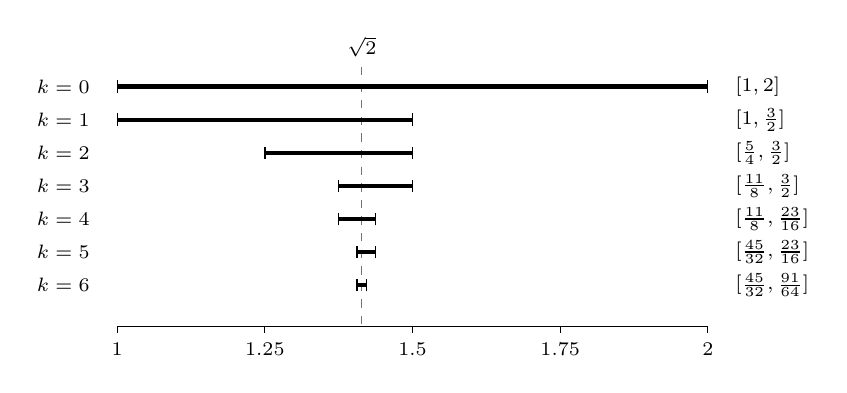
\begin{tikzpicture}[font=\scriptsize, x=7.5cm, y=1cm]
\draw[black!55, dashed, line width=0.4pt] (0.41421,0.25) -- (0.41421,-3.05);
\node[above, black] at (0.41421,0.25) {$\sqrt2$};
\foreach \k/\a/\b/\l in {0/0/1/{$[1,2]$}, 1/0/0.5/{$[1,\frac32]$}, 2/0.25/0.5/{$[\frac54,\frac32]$}, 3/0.375/0.5/{$[\frac{11}8,\frac32]$}, 4/0.375/0.4375/{$[\frac{11}8,\frac{23}{16}]$}, 5/0.40625/0.4375/{$[\frac{45}{32},\frac{23}{16}]$}, 6/0.40625/0.421875/{$[\frac{45}{32},\frac{91}{64}]$}} {
  \draw[line width=1.6pt] (\a,-0.42*\k) -- (\b,-0.42*\k);
  \draw[line width=0.5pt] (\a,-0.42*\k-0.08) -- (\a,-0.42*\k+0.08);
  \draw[line width=0.5pt] (\b,-0.42*\k-0.08) -- (\b,-0.42*\k+0.08);
  \node[anchor=east] at (-0.03,-0.42*\k) {$k=\k$};
  \node[anchor=west] at (1.03,-0.42*\k) {\l};}
\draw[line width=0.4pt] (0,-3.05) -- (1,-3.05);
\foreach \t/\l in {0/1, 0.25/1.25, 0.5/1.5, 0.75/1.75, 1/2} {\draw[line width=0.4pt] (\t,-3.05) -- (\t,-3.13); \node[below] at (\t,-3.13) {\l};}
\end{tikzpicture}}{Nested intervals for $\sqrt2$. Each interval $[a_k,b_k]$ is the half of the previous one that contains $\sqrt2$, decided by the sign of $m^2-2$ at the midpoint $m$. The lengths are $2^{-k}$, and the intervals close in on $\sqrt2=1.41421\ldots$ (dashed line).\label{fig:nested-sqrt2}}
\end{figure}

\subsection{Subsequences and the Bolzano--Weierstrass Theorem}

A bounded sequence need not converge, but it cannot avoid having convergent parts. To make this precise we need subsequences: the sequences obtained by keeping infinitely many terms, in their original order, and discarding the rest.

\begin{definition}[Subsequence]
\label{def:subsequence}
Let $(a_n)$ be a sequence and let $n_0<n_1<n_2<\cdots$ be a strictly increasing sequence of natural numbers. The sequence $(a_{n_k})_{k\in\mathbb N}=(a_{n_0},a_{n_1},a_{n_2},\ldots)$ is a \term{subsequence} of $(a_n)$.
\end{definition}

For example, $(a_{2k})=(a_0,a_2,a_4,\ldots)$ and $(a_{2k+1})$ are the subsequences of the terms with even and with odd index. A strictly increasing sequence of natural numbers satisfies $n_k\ge k$ for every $k$, by induction: $n_0\ge0$, and $n_{k+1}>n_k\ge k$ gives $n_{k+1}\ge k+1$. So a subsequence runs through the indices at least as fast as the original sequence, and this is all that the following proof needs.

\begin{proposition}
\label{prop:subsequence}
If $a_n\to L$, then every subsequence of $(a_n)$ converges to $L$. If $a_n\to\infty$, then every subsequence diverges to $\infty$.
\end{proposition}

\begin{proof}
Let $\varepsilon>0$ and choose $N$ with $|a_n-L|<\varepsilon$ for $n\ge N$. For $k\ge N$ we have $n_k\ge k\ge N$, so $|a_{n_k}-L|<\varepsilon$. The second statement is proved in the same way.
\end{proof}

The proposition gives the most convenient test for divergence: a sequence with two subsequences that converge to different limits diverges. The subsequences $(a_{2k})$ and $(a_{2k+1})$ of $\bigl((-1)^n\bigr)$ are constant, equal to $1$ and to $-1$, which gives a second proof that $(-1)^n$ diverges. The converse question is whether a divergent sequence has convergent subsequences at all. The sequence $(n)$ has none, since every subsequence is unbounded. For bounded sequences the answer is positive, and the proof uses a combinatorial lemma.

\begin{lemma}[Monotone subsequences]
\label{lem:monotone-subsequence}
Every sequence of real numbers has a monotone subsequence.
\end{lemma}

\begin{proof}
Call an index $n$ a \emph{peak} of the sequence $(a_n)$ if $a_n\ge a_m$ for all $m>n$, that is, if no later term is larger; from a peak, the view to the right is unobstructed. Suppose first that there are infinitely many peaks, $n_0<n_1<n_2<\cdots$. Since each $n_k$ is a peak and $n_{k+1}>n_k$, we have $a_{n_k}\ge a_{n_{k+1}}$, so $(a_{n_k})$ is a decreasing subsequence. Suppose next that there are only finitely many peaks, and let $n_0$ be larger than all of them. Since $n_0$ is not a peak, some $n_1>n_0$ satisfies $a_{n_1}>a_{n_0}$; since $n_1$ is not a peak either, some $n_2>n_1$ satisfies $a_{n_2}>a_{n_1}$; continuing in this way (formally, by recursion, choosing each time the smallest such index) we obtain a strictly increasing subsequence.
\end{proof}

The argument with peaks is standard~\cite{bartle2011}. The lemma is the infinite counterpart of the theorem of Erd\H{o}s and Szekeres (\cref{thm:erdos-szekeres}), which finds long monotone subsequences in long finite sequences. Combined with the monotone convergence theorem, it yields one of the central theorems of analysis. The theorem bears the names of Bolzano, whose paper of 1817 used a halving argument like that of the second proof below, and of Weierstrass, who made it a standard tool of analysis in his lectures~\cite{russ1980,hairer1996analysis}.

\begin{theorem}[Bolzano--Weierstrass]
\label{thm:bolzano-weierstrass}
Every bounded sequence of real numbers has a convergent subsequence. If all terms lie in a closed bounded interval $[c,d]$, the limit of the subsequence lies in $[c,d]$.
\end{theorem}

\begin{proof}
By \cref{lem:monotone-subsequence} the sequence has a monotone subsequence, which is bounded because the whole sequence is. By the monotone convergence theorem, this subsequence converges. If $c\le a_n\le d$ for all $n$, then the terms of the subsequence satisfy the same inequalities, and so does its limit, by \cref{prop:limit-order}\,(ii).
\end{proof}

There is a second proof, closer to the method of \cref{fig:nested-sqrt2}, which deserves to be known because it generalises to points in the plane and in space. Suppose all terms lie in $I_0=[c,d]$. Halve the interval; at least one of the two halves contains $a_n$ for infinitely many indices $n$, and we call it $I_1$. Halve $I_1$, and choose a half $I_2$ that again contains terms with infinitely many indices; and so on. By the nested interval theorem the intervals $I_k$, whose lengths are $(d-c)/2^k$, close in on a number $x$. Choosing indices $n_0<n_1<\cdots$ with $a_{n_k}\in I_k$, which is possible because each $I_k$ contains terms with arbitrarily large indices, gives a subsequence with $|a_{n_k}-x|\le(d-c)/2^k$, so $a_{n_k}\to x$.

Both proofs are nonconstructive in the sense of \cref{sec:existence}. The sequence $(\sin n)$ is bounded, so it has a convergent subsequence, but the theorem does not tell us which indices to choose or what the limit is; the second proof even asks at each step which half contains infinitely many terms, a question that no finite computation can answer in general. The theorem is nevertheless indispensable, because it converts the mere boundedness of a sequence into the existence of a point at which a subsequence accumulates. \Cref{sec:evt,sec:uniform} use it in exactly this way to prove the existence of maxima and the uniform continuity of continuous functions.

\subsection{Cauchy Sequences}

To verify the definition of convergence, one must know the limit. Often one does not, and it would be useful to recognise convergence from the terms alone. A convergent sequence has the property that its terms come close to each other, since they all come close to the limit. Remarkably, in $\mathbb R$ this property suffices.

\begin{definition}[Cauchy sequence]
\label{def:cauchy}
A sequence $(a_n)$ is a \term{Cauchy sequence} if
\[
\forall\varepsilon>0,\ \exists N\in\mathbb N,\ \forall m,n\ge N:\quad|a_m-a_n|<\varepsilon .
\]
\end{definition}

\begin{theorem}[Cauchy criterion]
\label{thm:cauchy-criterion}
A sequence of real numbers converges if and only if it is a Cauchy sequence.
\end{theorem}

\begin{proof}
Suppose $a_n\to L$ and let $\varepsilon>0$. Choose $N$ with $|a_n-L|<\varepsilon/2$ for $n\ge N$. For $m,n\ge N$, the triangle inequality gives $|a_m-a_n|\le|a_m-L|+|L-a_n|<\varepsilon$.

Conversely, let $(a_n)$ be a Cauchy sequence. It is bounded: with $\varepsilon=1$ there is $N$ with $|a_n-a_N|<1$ for all $n\ge N$, so $|a_n|<|a_N|+1$ for $n\ge N$, and the finitely many earlier terms are bounded by their maximum absolute value, as in the proof of \cref{prop:convergent-bounded}. By the Bolzano--Weierstrass theorem, some subsequence $(a_{n_k})$ converges, say to $L$. We show that the whole sequence converges to $L$. Let $\varepsilon>0$, and choose $N$ with $|a_m-a_n|<\varepsilon/2$ for all $m,n\ge N$. Choose $k$ so large that $n_k\ge N$ and $|a_{n_k}-L|<\varepsilon/2$. For every $n\ge N$,
\[
|a_n-L|\le|a_n-a_{n_k}|+|a_{n_k}-L|<\frac\varepsilon2+\frac\varepsilon2=\varepsilon .
\]
\end{proof}

The criterion goes back to Bolzano, who stated it in 1817, and to Cauchy, who used it in his \emph{Cours d'analyse} of 1821~\cite{russ1980,cauchy1821,grabiner1981}. Its value lies in the fact that it refers only to the terms. Two examples illustrate it, one positive and one negative.

The partial sums $s_n=\sum_{k=1}^n1/k^2$ form a Cauchy sequence. For $m>n\ge1$, the estimate used above gives
\[
0<s_m-s_n=\sum_{k=n+1}^m\frac1{k^2}<\sum_{k=n+1}^m\Bigl(\frac1{k-1}-\frac1k\Bigr)=\frac1n-\frac1m<\frac1n ,
\]
so $|s_m-s_n|<\varepsilon$ for all $m,n\ge N$ once $1/N<\varepsilon$. This proves again that $(s_n)$ converges, without using monotonicity.

The harmonic numbers $H_n=\sum_{k=1}^n1/k$ do not form a Cauchy sequence. The sum $H_{2n}-H_n$ has $n$ terms $1/k$ with $n<k\le2n$, each at least $1/(2n)$, so
\[
H_{2n}-H_n\ge n\cdot\frac1{2n}=\frac12\qquad(n\ge1).
\]
With $\varepsilon=\frac12$ no $N$ can work, since $m=2N$ and $n=N$ violate the condition. Hence $(H_n)$ diverges, and since it is increasing, $H_n\to\infty$ by \cref{cor:monotone-dichotomy}. This is the fact announced in \cref{sec:recurrences}, and Chapter~8 shows that $H_n$ grows like $\ln n$.

The second example carries a warning for computation. The steps $H_{n+1}-H_n=1/(n+1)$ tend to zero, and an iterative program that stops as soon as two consecutive values differ by less than a tolerance would stop on the harmonic numbers, reporting a ``limit'' that does not exist. The Cauchy condition requires that \emph{all} pairs of late terms be close, not only consecutive ones. A test on consecutive differences is justified only when something more is known about the sequence, for instance a bound such as \eqref{eq:heron-error}, which shows that for Heron's method the error after a step is far smaller than the step itself.

In $\mathbb Q$, Cauchy sequences need not converge: the iterates of \cref{tab:heron} form a Cauchy sequence of rational numbers whose limit is irrational. Cantor's construction of the real numbers, outlined in the note at the end of \cref{sec:reals}, turns this observation into a definition, and Volume~II uses Cauchy sequences to define completeness for general metric spaces.

\begin{note}{Equivalent forms of completeness}
In an ordered field the following statements are equivalent: (a) every nonempty set that is bounded above has a supremum; (b) every bounded monotone sequence converges; (c) every bounded sequence has a convergent subsequence; (d) the field is Archimedean, and every Cauchy sequence converges; (e) the field is Archimedean, and every nested sequence of closed bounded intervals has a nonempty intersection. The proofs of this section show that (a) implies (b), that (b) implies (c) and the nested interval property, and that (c) implies the convergence of Cauchy sequences; (c) also implies the Archimedean property, since otherwise the sequence $0,1,2,\ldots$ would be bounded, and its subsequences, whose consecutive terms differ by at least $1$, cannot converge. The remaining implications, which close the circle, are discussed by Propp~\cite{propp2013}, who also explains why the Archimedean property cannot be omitted from (d) and (e): there are ordered fields that are not Archimedean in which every Cauchy sequence converges (the field of formal Laurent series is one), and others in which every nested sequence of closed bounded intervals has a common point (Propp uses a field of surreal numbers); neither kind of field satisfies (a). By contrast, (b) and (c) imply (a) in every ordered field, without a separate Archimedean hypothesis. Any of the five statements may therefore serve as the completeness axiom of the real numbers, and textbooks differ in their choice~\cite{bartle2011,abbott2015}. Constructive mathematics prefers (d) together with explicit rates of convergence, as remarked in \cref{ch:numbers}.
\end{note}

\section{Limits of Functions}
\label{sec:function-limits}

The limit of a function describes how its values behave as the argument approaches a point. \Cref{def:limit} introduced it for functions defined on an open interval around the point, except possibly at the point itself, and \cref{fig:epsilon-delta} showed one round of the game that the definition describes. This section extends the definition to more general domains, relates limits of functions to limits of sequences and transfers the limit laws, and it computes the most important limit of trigonometry, $\lim_{x\to0}(\sin x)/x=1$.

\subsection{The Definition}

Many functions of interest are not defined on a whole open interval around every point that matters. The square root is defined on $[0,\infty)$, and we want to speak of its behaviour as $x$ approaches $0$ from the right; a function may be defined only on the set $\{1/n: n\ge1\}$, and we may ask what happens as $x$ approaches $0$ through this set. What the definition really needs is that the function be defined at points arbitrarily close to $a$, other than $a$ itself.

\begin{definition}[Accumulation point]
\label{def:accumulation}
Let $D\subseteq\mathbb R$. A real number $a$ is an \term{accumulation point} of $D$ if for every $\delta>0$ there is a point $x\in D$ with $0<|x-a|<\delta$. A point of $D$ that is not an accumulation point of $D$ is an \term{isolated point} of $D$.
\end{definition}

An accumulation point of $D$ may or may not belong to $D$. Every point of $[a,b]$ is an accumulation point of the open interval $(a,b)$, when $a<b$; the number $0$ is an accumulation point of $\{1/n: n\ge1\}$ but not an element of it; and every integer is an isolated point of $\mathbb Z$, since $(k-\frac12,k+\frac12)$ contains no other integer.

\begin{definition}[Limit of a function]
\label{def:function-limit}
Let $f\colon D\to\mathbb R$ be a function, $a$ an accumulation point of $D$ and $L$ a real number. Then $f(x)$ \term{tends to} $L$ as $x$ tends to $a$, written $\lim_{x\to a}f(x)=L$ or $f(x)\to L$ as $x\to a$, if
\begin{equation}
\forall\varepsilon>0,\ \exists\delta>0,\ \forall x\in D:\quad0<|x-a|<\delta\ \Rightarrow\ |f(x)-L|<\varepsilon .
\label{eq:function-limit}
\end{equation}
\end{definition}

When $D$ contains an open interval around $a$ with the point $a$ possibly removed, this is \cref{def:limit}. Everything said there applies: $\delta$ may depend on $\varepsilon$ but not on $x$, and the value of $f$ at $a$, if there is one, plays no role. The requirement that $a$ be an accumulation point is not a technicality. If some interval $(a-\delta,a+\delta)$ contained no point of $D$ other than $a$, the implication in \eqref{eq:function-limit} would hold vacuously for this $\delta$, whatever $L$ is, and every number would be a limit. With the requirement, the limit is unique.

\begin{proposition}
\label{prop:function-limit-unique}
If $\lim_{x\to a}f(x)=L$ and $\lim_{x\to a}f(x)=M$, then $L=M$.
\end{proposition}

\begin{proof}
Let $\varepsilon>0$, and let $\delta_1$ and $\delta_2$ be the numbers that \eqref{eq:function-limit} provides for $L$ and for $M$. Since $a$ is an accumulation point of $D$, there is $x\in D$ with $0<|x-a|<\min(\delta_1,\delta_2)$, and for it $|L-M|\le|L-f(x)|+|f(x)-M|<2\varepsilon$. As in the proof of \cref{thm:limit-unique}, a nonnegative number smaller than $2\varepsilon$ for every $\varepsilon>0$ is zero.
\end{proof}

\emph{Examples.} We have $\lim_{x\to2}x^2=4$. To find $\delta$ we factor: $|x^2-4|=|x-2|\,|x+2|$. The factor $|x-2|$ is small when $x$ is close to $2$; the factor $|x+2|$ is not small, but it is bounded near $2$: if $|x-2|<1$, then $1<x<3$ and $|x+2|<5$. So for $|x-2|<\delta\coloneqq\min(1,\varepsilon/5)$ we get $|x^2-4|<5\cdot\varepsilon/5=\varepsilon$. The device of first restricting $x$ to a fixed neighbourhood of $a$, to bound the factors that do not become small, is the standard technique for nonlinear functions.

The function $f(x)=(x^2-1)/(x-1)$ is not defined at $1$. For $x\ne1$, however, $f(x)=x+1$, and since the limit ignores the point $1$ itself, $\lim_{x\to1}f(x)=\lim_{x\to1}(x+1)=2$, with $\delta=\varepsilon$. Limits of this kind, where substituting $x=a$ gives the meaningless expression $0/0$, are the subject of differential calculus: every derivative is one.

Similarly, on the domain $D=[0,\infty)\setminus\{4\}$,
\[
\frac{\sqrt x-2}{x-4}=\frac{\sqrt x-2}{(\sqrt x-2)(\sqrt x+2)}=\frac1{\sqrt x+2}
\]
and
\[
\Bigl|\frac1{\sqrt x+2}-\frac14\Bigr|=\frac{|\sqrt x-2|}{4(\sqrt x+2)}=\frac{|x-4|}{4(\sqrt x+2)^2}\le\frac{|x-4|}{16},
\]
so the quotient tends to $\frac14$ as $x\to4$, with $\delta=16\varepsilon$.

\subsection{Limits along Sequences}

The next theorem connects limits of functions with limits of sequences. It says that $f(x)\to L$ as $x\to a$ exactly when $f(x_n)\to L$ for every way of approaching $a$ along a sequence. This allows us to transfer the results of \cref{sec:limit-laws} to functions without proving them again, and it is the most convenient way to show that a limit does not exist~\cite{abbott2015}.

\begin{theorem}[Sequential characterisation of limits]
\label{thm:sequential-limit}
Let $f\colon D\to\mathbb R$ and let $a$ be an accumulation point of $D$. Then $\lim_{x\to a}f(x)=L$ if and only if $f(x_n)\to L$ for every sequence $(x_n)$ of points of $D\setminus\{a\}$ with $x_n\to a$.
\end{theorem}

\begin{proof}
Suppose $\lim_{x\to a}f(x)=L$, and let $(x_n)$ be a sequence in $D\setminus\{a\}$ with $x_n\to a$. Given $\varepsilon>0$, choose $\delta$ by \eqref{eq:function-limit}, and then $N$ with $|x_n-a|<\delta$ for all $n\ge N$. For these $n$ we have $0<|x_n-a|<\delta$, since $x_n\ne a$, and therefore $|f(x_n)-L|<\varepsilon$.

We prove the converse by contraposition. Suppose $\lim_{x\to a}f(x)=L$ is false. Negating \eqref{eq:function-limit} as in \eqref{eq:not-limit}, there is $\varepsilon>0$ such that for every $\delta>0$ some $x\in D$ satisfies $0<|x-a|<\delta$ and $|f(x)-L|\ge\varepsilon$. Apply this with $\delta=1/(n+1)$ for each $n\in\mathbb N$, and call the point obtained $x_n$. Then $x_n\in D\setminus\{a\}$ and $|x_n-a|<1/(n+1)$, so $x_n\to a$ by the squeeze theorem; but $|f(x_n)-L|\ge\varepsilon$ for every $n$, so $f(x_n)\not\to L$.
\end{proof}

The theorem gives a test for the nonexistence of a limit: if two sequences $x_n\to a$ and $y_n\to a$ in $D\setminus\{a\}$ give $f(x_n)$ and $f(y_n)$ different limits, or if one sequence gives values that do not converge, then $\lim_{x\to a}f(x)$ does not exist. The standard example is $f(x)=\sin(1/x)$ on $D=\mathbb R\setminus\{0\}$, which oscillates between $-1$ and $1$ infinitely often near $0$ (\cref{fig:discontinuities}D). With $x_n\coloneqq1/(n\pi)$ and $y_n\coloneqq1/(2n\pi+\pi/2)$ for $n\ge1$, both sequences tend to $0$, while $f(x_n)=\sin(n\pi)=0$ and $f(y_n)=\sin(2n\pi+\pi/2)=1$ for every $n$, by the values of the sine recalled in \cref{asm:trig-geometry} below. So $\sin(1/x)$ has no limit as $x\to0$.

\begin{theorem}[Limit laws for functions]
\label{thm:function-limit-laws}
Let $f,g\colon D\to\mathbb R$, let $a$ be an accumulation point of $D$, and suppose $\lim_{x\to a}f(x)=L$ and $\lim_{x\to a}g(x)=M$. Then:
\begin{enumerate}
\item $\lim_{x\to a}\bigl(f(x)+g(x)\bigr)=L+M$, $\lim_{x\to a}cf(x)=cL$ for every real $c$, and $\lim_{x\to a}f(x)g(x)=LM$;
\item if $M\ne0$, then there is $\delta>0$ with $g(x)\ne0$ for all $x\in D$ with $0<|x-a|<\delta$, and $\lim_{x\to a}f(x)/g(x)=L/M$, the quotient being considered on the set of those $x\in D$ with $g(x)\ne0$;
\item if $f(x)\le g(x)$ for all $x\in D\setminus\{a\}$ in some interval around $a$, then $L\le M$;
\item (squeeze theorem) if $h\colon D\to\mathbb R$ satisfies $f(x)\le h(x)\le g(x)$ for all $x\in D\setminus\{a\}$ in some interval around $a$, and $L=M$, then $\lim_{x\to a}h(x)=L$.
\end{enumerate}
\end{theorem}

\begin{proof}
Each statement follows from the corresponding statement for sequences and \cref{thm:sequential-limit}. For the product, for instance, let $x_n\to a$ with $x_n\in D\setminus\{a\}$; then $f(x_n)\to L$ and $g(x_n)\to M$, so $f(x_n)g(x_n)\to LM$ by \cref{thm:limit-laws}\,(iii), and since the sequence was arbitrary, $f(x)g(x)\to LM$. In (ii), \eqref{eq:function-limit} for $g$ with $\varepsilon=|M|/2$ gives a $\delta$ with $|g(x)|>|M|/2>0$ for $0<|x-a|<\delta$; so $a$ is an accumulation point of the set where $g\ne0$, and the sequential argument applies to the quotient. Parts (iii) and (iv) follow in the same way from \cref{prop:limit-order}\,(ii) and \cref{thm:squeeze}, applied to sequences whose terms lie in the given interval, as all terms of a sequence converging to $a$ eventually do.
\end{proof}

Since $\lim_{x\to a}x=a$ and $\lim_{x\to a}c=c$, with $\delta=\varepsilon$ and with any $\delta$, part (i) gives $\lim_{x\to a}p(x)=p(a)$ for every polynomial $p$, and part (ii) gives $\lim_{x\to a}p(x)/q(x)=p(a)/q(a)$ for polynomials $p$ and $q$ with $q(a)\ne0$. The squeeze theorem gives, for example, $\lim_{x\to0}x\sin(1/x)=0$, because $-|x|\le x\sin(1/x)\le|x|$ for $x\ne0$. The factor $x$ tames the oscillation of $\sin(1/x)$, which has no limit.

\subsection{One-Sided Limits}

A function may approach different values from the two sides of a point. The step function $H$ of \cref{prop:step-limit} is $0$ to the left of $0$ and $1$ to the right, and its limit at $0$ does not exist (\cref{prop:step-no-limit}); yet its behaviour on each side separately is as simple as can be. One-sided limits capture this behaviour. They are limits of restrictions of $f$ (\cref{def:restriction}).

\begin{definition}[One-sided limits]
\label{def:one-sided}
Let $f\colon D\to\mathbb R$. If $a$ is an accumulation point of $D\cap(a,\infty)$, the \term{right-hand limit} of $f$ at $a$ is
\[
\lim_{x\to a^+}f(x)\coloneqq\lim_{x\to a}f|_{D\cap(a,\infty)}(x),
\]
provided the limit on the right exists. If $a$ is an accumulation point of $D\cap(-\infty,a)$, the \term{left-hand limit} $\lim_{x\to a^-}f(x)$ is defined in the same way with $D\cap(-\infty,a)$. We also write $f(a^+)$ and $f(a^-)$ for the one-sided limits, and $x\to a^+$ and $x\to a^-$ are read ``$x$ tends to $a$ from the right'' and ``from the left''.
\end{definition}

Explicitly, $\lim_{x\to a^+}f(x)=L$ means that for every $\varepsilon>0$ there is $\delta>0$ with $|f(x)-L|<\varepsilon$ for all $x\in D$ with $a<x<a+\delta$. The notation $f(a^+)$ is convenient but must be read with care: it is a limit and not a value of $f$, and it may differ from $f(a)$ or exist when $f(a)$ does not.

\begin{proposition}
\label{prop:one-sided-limits}
Let $f\colon D\to\mathbb R$, and let $a$ be an accumulation point of both $D\cap(a,\infty)$ and $D\cap(-\infty,a)$. Then $\lim_{x\to a}f(x)=L$ if and only if both one-sided limits exist and are equal to $L$.
\end{proposition}

\begin{proof}
If $\lim_{x\to a}f(x)=L$, the $\delta$ that works for $f$ also works for both restrictions. Conversely, if $\delta_1$ works for the right-hand limit and $\delta_2$ for the left-hand limit, then $\min(\delta_1,\delta_2)$ works for $f$, since every $x$ with $0<|x-a|<\delta$ lies on one of the two sides.
\end{proof}

For the step function, $H(0^-)=0$ and $H(0^+)=1$, and the proposition explains once more why $\lim_{x\to0}H(x)$ does not exist. The floor function satisfies $\lfloor k^-\rfloor=k-1$ and $\lfloor k^+\rfloor=k$ at every integer $k$, since $\lfloor x\rfloor=k-1$ for $k-1\le x<k$ and $\lfloor x\rfloor=k$ for $k\le x<k+1$. The sign of $x$, written as $x/|x|$ for $x\ne0$, has the one-sided limits $-1$ and $1$ at $0$. For the square root on $D=[0,\infty)$, only the right-hand limit at $0$ makes sense, and it coincides with $\lim_{x\to0}\sqrt x$ in the sense of \cref{def:function-limit}, which equals $0$: given $\varepsilon$, take $\delta=\varepsilon^2$, so that $0\le x<\varepsilon^2$ implies $\sqrt x<\varepsilon$ by \cref{prop:ineq-rules}\,(iii).

\subsection{Infinite Limits and Limits at Infinity}

As for sequences, we want to say that a function grows beyond all bounds near a point, or that it approaches a number as its argument grows beyond all bounds.

\begin{definition}[Limits involving infinity]
\label{def:limits-infinity}
Let $f\colon D\to\mathbb R$.
\begin{enumerate}
\item If $D$ is not bounded above, $\lim_{x\to\infty}f(x)=L$ means: for every $\varepsilon>0$ there is $R$ such that $|f(x)-L|<\varepsilon$ for all $x\in D$ with $x>R$. The limit $\lim_{x\to-\infty}f(x)=L$, for $D$ not bounded below, is defined in the same way with $x<R$.
\item If $a$ is an accumulation point of $D$, $\lim_{x\to a}f(x)=\infty$ means: for every $M$ there is $\delta>0$ such that $f(x)>M$ for all $x\in D$ with $0<|x-a|<\delta$; and $\lim_{x\to a}f(x)=-\infty$ means that $\lim_{x\to a}(-f(x))=\infty$.
\item If $D$ is not bounded above, $\lim_{x\to\infty}f(x)=\infty$ means: for every $M$ there is $R$ such that $f(x)>M$ for all $x\in D$ with $x>R$.
\end{enumerate}
The remaining combinations, such as one-sided infinite limits $\lim_{x\to a^+}f(x)=\infty$ or the limit $\lim_{x\to-\infty}f(x)=\infty$, are defined analogously.
\end{definition}

In each case the pattern is the same as before: a tolerance or a level is given, and a neighbourhood of $a$, or a half-line $(R,\infty)$ standing for a ``neighbourhood of infinity'', must be found on which the values meet it. For example, $\lim_{x\to\infty}1/x=0$ with $R=1/\varepsilon$, and
\[
\lim_{x\to\infty}\frac{2x^2+1}{x^2+3}=\lim_{x\to\infty}\frac{2+1/x^2}{1+3/x^2}=2 ,
\]
by the limit laws, which hold for limits at infinity with the same proofs. Near $0$, $1/x^2\to\infty$, while $1/x\to\infty$ as $x\to0^+$ and $1/x\to-\infty$ as $x\to0^-$ (\cref{fig:discontinuities}C). If $\lim_{x\to a^+}f(x)$ or $\lim_{x\to a^-}f(x)$ is infinite, the line $x=a$ is a \term{vertical asymptote} of the graph of $f$; if $\lim_{x\to\infty}f(x)=L$ or $\lim_{x\to-\infty}f(x)=L$, the line $y=L$ is a \term{horizontal asymptote}.

The sequential characterisation also holds in these settings, with the same proof; for limits at infinity it reads: $\lim_{x\to\infty}f(x)=L$ if and only if $f(x_n)\to L$ for every sequence $(x_n)$ in $D$ with $x_n\to\infty$. In particular, if $\lim_{x\to\infty}f(x)=L$ and $D$ contains the natural numbers, then $f(n)\to L$. The converse is false: $f(x)=\sin(\pi x)$ satisfies $f(n)=0$ for every integer $n$, but $f(2n+\frac12)=\sin(2n\pi+\frac\pi2)=1$ for every integer $n$, by \cref{asm:trig-geometry}\,(ii) below, so $\lim_{x\to\infty}f(x)$ does not exist. A sequence samples a function only at particular points, and it may miss what happens in between.

\subsection{The Limit of \texorpdfstring{$(\sin x)/x$}{sin(x)/x}}

The derivative of the sine at $0$ is the limit of $(\sin x)/x$ as $x\to0$, and the derivatives of all trigonometric functions are derived from this limit in Chapter~6. A rigorous treatment of the trigonometric functions must wait until Chapter~9, which defines them by power series; here, as in \cref{ch:numbers}, we take the following facts from school geometry.

\begin{assumption}[Trigonometric facts from geometry]
\label{asm:trig-geometry}
In addition to \cref{asm:trig}, the sine and cosine satisfy:
\begin{enumerate}
\item $\sin(-x)=-\sin x$ and $\cos(-x)=\cos x$ for all real $x$;
\item $\sin(\pi/2)=1$, $\sin(k\pi)=0$ for every integer $k$, $\sin(x+2\pi)=\sin x$ for all $x$, and $\pi>3$;
\item if $0<x<\pi/2$, then $\sin x>0$ and $\cos x>0$, and the sector of the unit disc between the angles $0$ and $x$ has area $x/2$;
\item $\sin$ is strictly increasing on $[-\pi/2,\pi/2]$, $\cos$ is strictly decreasing on $[0,\pi]$, and $\tan=\sin/\cos$ is strictly increasing on $(-\pi/2,\pi/2)$.
\end{enumerate}
\end{assumption}

Chapter~9 proves all of these from the definitions; in particular, the area of a sector, which school geometry takes for granted, is computed there by an integral.

\begin{lemma}
\label{lem:sin-bounds}
For $0<x<\pi/2$,
\[
\sin x<x<\tan x .
\]
Consequently $|\sin x|\le|x|$ for every real number $x$, with equality only for $x=0$.
\end{lemma}

\begin{proof}
Let $O=(0,0)$, $A=(1,0)$, $P=(\cos x,\sin x)$ and $T=(1,\tan x)$, as in \cref{fig:sin-area}. The point $P$ lies on the unit circle at angle $x$, and $T$ is the point where the ray from $O$ through $P$ meets the vertical line through $A$, since $T=P/\cos x$. The triangle $OAP$ lies inside the sector $OAP$, which lies inside the triangle $OAT$, and each region is strictly smaller than the next. The triangle $OAP$ has base $OA=1$ and height $\sin x$, the sector has area $x/2$ by \cref{asm:trig-geometry}\,(iii), and the triangle $OAT$ has base $1$ and height $\tan x$. Hence $\frac12\sin x<\frac12x<\frac12\tan x$. (Besides \cref{asm:trig-geometry}\,(iii), the argument uses two further facts of school geometry: the area of a triangle is half its base times its height, and a region that lies inside another and misses part of it has the smaller area. Chapter~9 proves the inequality $\sin x<x<\tan x$ directly from the definitions.)

For the consequence, the case $0<x<\pi/2$ has just been shown, with strict inequality. If $x\ge\pi/2$, then $|\sin x|\le1<\pi/2\le x$ by \cref{asm:trig}\,(i) and $\pi>3$. For $x<0$ apply these cases to $-x$ and use $|\sin(-x)|=|\sin x|$; and $\sin0=0$.
\end{proof}

\begin{figure}
\sdfloat{%
\begin{tikzpicture}[font=\scriptsize, scale=3.4]
\fill[sdfill] (0,0) -- (1,0) arc[start angle=0, end angle=40, radius=1] -- cycle;
\draw[line width=0.4pt] (-0.08,0) -- (1.15,0);
\draw[line width=0.4pt] (0,-0.08) -- (0,0.95);
\draw[line width=0.5pt] (1,0) arc[start angle=0, end angle=80, radius=1];
\draw[line width=0.7pt] (0,0) -- (1,0.8391) -- (1,0) -- cycle;
\draw[line width=0.7pt] (0.766,0.6428) -- (1,0);
\draw[black!55, dashed, line width=0.4pt] (0.766,0.6428) -- (0.766,0);
\fill (0,0) circle (0.4pt) (1,0) circle (0.4pt) (0.766,0.6428) circle (0.4pt) (1,0.8391) circle (0.4pt);
\node[below left] at (0,0) {$O$};
\node[below right] at (1,0) {$A$};
\node[above left] at (0.766,0.6428) {$P$};
\node[right] at (1,0.8391) {$T$};
\draw[line width=0.4pt] (0.22,0) arc[start angle=0, end angle=40, radius=0.22];
\node at (0.3,0.1) {$x$};
\node[right] at (1,0.42) {$\tan x$};
\node[left] at (0.766,0.24) {$\sin x$};
\node[below] at (0.766,0) {$\cos x$};
\end{tikzpicture}}{The inequality $\sin x<x<\tan x$ for $0<x<\pi/2$, here $x=40^\circ$. The triangle $OAP$, of area $\frac12\sin x$, lies inside the circular sector $OAP$ (shaded), of area $\frac12x$, which lies inside the triangle $OAT$, of area $\frac12\tan x$.\label{fig:sin-area}}
\end{figure}

\begin{proposition}
\label{prop:sin-limit}
\[
\lim_{x\to0}\frac{\sin x}x=1\qquad\text{and}\qquad\lim_{x\to0}\frac{1-\cos x}{x^2}=\frac12 .
\]
\end{proposition}

\begin{proof}
For $0<x<\pi/2$, \cref{lem:sin-bounds} gives $\sin x<x$, that is, $(\sin x)/x<1$, and $x<\sin x/\cos x$, that is, $\cos x<(\sin x)/x$, after multiplying by the positive number $(\cos x)/x$. All three members of $\cos x<(\sin x)/x<1$ are even functions of $x$, by \cref{asm:trig-geometry}\,(i), so the inequalities hold for $0<|x|<\pi/2$.

It remains to show that $\cos x\to1$. By the addition formula of \cref{asm:trig}\,(ii) with $\alpha=\beta=x/2$, and by (i) there, $\cos x=\cos^2(x/2)-\sin^2(x/2)=1-2\sin^2(x/2)$. Hence, by \cref{lem:sin-bounds},
\begin{equation}
0\le1-\cos x=2\sin^2\frac x2\le2\Bigl(\frac x2\Bigr)^2=\frac{x^2}2 ,
\label{eq:one-minus-cos}
\end{equation}
and the squeeze theorem gives $\cos x\to1$. Applying the squeeze theorem to $\cos x<(\sin x)/x<1$ gives the first limit.

For the second, the same identity gives
\[
\frac{1-\cos x}{x^2}=\frac12\biggl(\frac{\sin(x/2)}{x/2}\biggr)^2 .
\]
If $x_n\to0$ with $x_n\ne0$, then $x_n/2\to0$, so $\sin(x_n/2)/(x_n/2)\to1$ by the first limit and \cref{thm:sequential-limit}; the limit laws then give $(1-\cos x_n)/x_n^2\to\frac12$, and \cref{thm:sequential-limit} once more gives the claim.
\end{proof}

Numerically, $\sin(0.1)/0.1=0.998334\ldots$ and $\sin(0.01)/0.01=0.99998333\ldots$; the deviation from $1$ is about $x^2/6$, as the Taylor expansion of Chapter~8 will explain. The two limits say that, for small $x$ measured in radians, $\sin x\approx x$ and $\cos x\approx1-x^2/2$, approximations used throughout physics and engineering. They depend on measuring angles in radians: with $x$ in degrees, $\sin x/x$ tends to $\pi/180$.

A word on logic. \Cref{sec:existence} warned that proving $\lim_{x\to0}(\sin x)/x=1$ with l'H\^opital's rule is circular, because the rule needs the derivative of the sine, which is computed from this very limit. The geometric proof above is not circular, provided that the area of a sector is known independently of the derivative of the sine; Chapter~9 provides such a foundation.

\section{Continuity}
\label{sec:continuity}

The informal idea of a continuous function is one whose graph can be drawn without lifting the pen. This idea is suggestive but inadequate: it gives no means of proof, it says nothing about functions defined on complicated sets, and it breaks down for functions such as $x\sin(1/x)$, whose graph near $0$ is infinitely long. The precise idea is that a small change of the argument produces only a small change of the value. For computation this is the essential property. Every input to a computation is known or stored only approximately, and a continuous function guarantees that the output is correspondingly close to the exact one; at a discontinuity of a function such as the floor or the sign, an arbitrarily small error in the input may change the output completely.

\subsection{The Definition}

\begin{definition}[Continuity]
\label{def:continuity}
Let $f\colon D\to\mathbb R$ and $a\in D$. The function $f$ is \term{continuous at} $a$ if
\begin{equation}
\forall\varepsilon>0,\ \exists\delta>0,\ \forall x\in D:\quad|x-a|<\delta\ \Rightarrow\ |f(x)-f(a)|<\varepsilon .
\label{eq:continuity}
\end{equation}
It is \term{continuous on} a set $S\subseteq D$ if it is continuous at every point of $S$, and \term{continuous} if it is continuous on $D$. The set of continuous functions $D\to\mathbb R$ is denoted $C(D)$, and for an interval $[a,b]$ we write $C[a,b]$.
\end{definition}

Compared with the definition of a limit, two things have changed: the point $a$ belongs to $D$, and the limit is required to be the value $f(a)$. The condition $0<|x-a|$ has been dropped, since for $x=a$ the inequality $|f(x)-f(a)|<\varepsilon$ holds anyway. If $a$ is an isolated point of $D$, some interval $(a-\delta,a+\delta)$ contains no point of $D$ other than $a$, and $f$ is continuous at $a$ automatically. Thus every function on $\mathbb N$ or on $\mathbb Z$, for instance every sequence regarded as a function on $\mathbb N$, is continuous; this is consistent, if not very interesting. At accumulation points, continuity is a statement about limits, and the following theorem collects three equivalent forms of it.

\begin{theorem}[Forms of continuity]
\label{thm:continuity-forms}
Let $f\colon D\to\mathbb R$ and $a\in D$. The following statements are equivalent.
\begin{enumerate}
\item $f$ is continuous at $a$.
\item For every sequence $(x_n)$ in $D$ with $x_n\to a$, $f(x_n)\to f(a)$.
\end{enumerate}
If $a$ is an accumulation point of $D$, they are also equivalent to
\begin{enumerate}
\setcounter{enumi}{2}
\item $\lim_{x\to a}f(x)=f(a)$.
\end{enumerate}
\end{theorem}

\begin{proof}
The equivalence of (i) and (ii) is proved exactly as \cref{thm:sequential-limit}; the only difference is that the sequence may now take the value $a$, at which $|f(x_n)-f(a)|=0$. If $a$ is an accumulation point, (i) and (iii) are equivalent because \eqref{eq:continuity} and \eqref{eq:function-limit} with $L=f(a)$ differ only at $x=a$, where \eqref{eq:continuity} holds trivially.
\end{proof}

Form (ii) says that continuous functions commute with limits: $f(\lim x_n)=\lim f(x_n)$. This is how continuity is used most often. We used it already, without saying so, when we passed to the limit in Heron's recursion: the map $x\mapsto\frac12(x+2/x)$ is continuous at $L>0$, by the results below.

\emph{Examples.} Constant functions and the identity $x\mapsto x$ are continuous, with any $\delta$ and with $\delta=\varepsilon$. The absolute value is continuous, since $\bigl||x|-|a|\bigr|\le|x-a|$ by the reverse triangle inequality, so $\delta=\varepsilon$ works. The square root is continuous on $[0,\infty)$: at $a=0$ this was shown in \cref{sec:function-limits}, and for $a>0$,
\[
|\sqrt x-\sqrt a|=\frac{|x-a|}{\sqrt x+\sqrt a}\le\frac{|x-a|}{\sqrt a},
\]
so $\delta=\varepsilon\sqrt a$ works. The sine and cosine are continuous on $\mathbb R$. From the addition formulas of \cref{asm:trig}\,(ii), applied to $u+v$ and $u-v$, together with \cref{asm:trig-geometry}\,(i), one obtains
\[
\sin(u+v)-\sin(u-v)=2\cos u\sin v,\qquad\cos(u+v)-\cos(u-v)=-2\sin u\sin v .
\]
With $u=(x+a)/2$ and $v=(x-a)/2$, and with $|\cos u|\le1$, $|\sin u|\le1$ and \cref{lem:sin-bounds},
\begin{equation}
|\sin x-\sin a|\le2\Bigl|\sin\frac{x-a}2\Bigr|\le|x-a|,\qquad|\cos x-\cos a|\le|x-a| ,
\label{eq:sin-lipschitz}
\end{equation}
so again $\delta=\varepsilon$ works. The step function $H$ is continuous at every $x\ne0$, where it is locally constant, and discontinuous at $0$; the floor function is continuous exactly at the non-integers.

\subsection{Combining Continuous Functions}

\begin{theorem}
\label{thm:continuity-algebra}
Let $f,g\colon D\to\mathbb R$ be continuous at $a\in D$, and let $c$ be a real number. Then $f+g$, $cf$ and $fg$ are continuous at $a$, and if $g(a)\ne0$, then $f/g$, defined on $\{x\in D: g(x)\ne0\}$, is continuous at $a$.
\end{theorem}

\begin{proof}
By \cref{thm:continuity-forms}, it suffices to check form (ii). If $x_n\to a$ in $D$, then $f(x_n)\to f(a)$ and $g(x_n)\to g(a)$, and the limit laws of \cref{thm:limit-laws} give $f(x_n)+g(x_n)\to f(a)+g(a)$, and so on. For the quotient the sequence $(x_n)$ is taken in the set where $g\ne0$.
\end{proof}

\begin{corollary}
\label{cor:rational-continuous}
Polynomials are continuous on $\mathbb R$. A rational function $p/q$, with polynomials $p$ and $q$, is continuous on the set $\{x: q(x)\ne0\}$. The tangent $\tan=\sin/\cos$ is continuous at every $x$ with $\cos x\ne0$.
\end{corollary}

\begin{proof}
Polynomials are built from constants and the identity by finitely many sums and products; apply \cref{thm:continuity-algebra} and induction on the number of operations. The other two statements follow from the quotient rule of the theorem.
\end{proof}

The third way of combining functions is composition, and here a direct $\varepsilon$--$\delta$ proof is instructive, because it shows how tolerances pass through a chain of computations.

\begin{theorem}[Continuity of compositions]
\label{thm:composition-continuous}
Let $f\colon D\to\mathbb R$ and $g\colon E\to\mathbb R$ with $f(D)\subseteq E$. If $f$ is continuous at $a\in D$ and $g$ is continuous at $f(a)$, then $g\circ f$ is continuous at $a$.
\end{theorem}

\begin{proof}
Let $\varepsilon>0$. Since $g$ is continuous at $b\coloneqq f(a)$, there is $\eta>0$ such that $|g(y)-g(b)|<\varepsilon$ for all $y\in E$ with $|y-b|<\eta$. Since $f$ is continuous at $a$, applied with the tolerance $\eta$, there is $\delta>0$ such that $|f(x)-b|<\eta$ for all $x\in D$ with $|x-a|<\delta$. For such $x$, the point $y=f(x)$ lies in $E$ and satisfies $|y-b|<\eta$, so $|g(f(x))-g(f(a))|<\varepsilon$.
\end{proof}

The proof runs backwards through the computation: the tolerance $\varepsilon$ demanded of the final result determines the tolerance $\eta$ that the intermediate result must meet, and $\eta$ determines the accuracy $\delta$ required of the input. Error analysis of numerical algorithms follows the same backward path, with explicit numbers in place of the existence of $\eta$ and $\delta$ (Volume~V).

The same argument gives a rule for limits of compositions: if $\lim_{x\to a}f(x)=b$, and $g$ is continuous at $b$, then
\begin{equation}
\lim_{x\to a}g(f(x))=g(b)=g\Bigl(\lim_{x\to a}f(x)\Bigr).
\label{eq:limit-composition}
\end{equation}
Continuity of $g$ at $b$ cannot be weakened to the existence of $\lim_{y\to b}g(y)$. Let $f(x)=0$ for all $x$, and let $g(0)=1$ and $g(y)=0$ for $y\ne0$. Then $\lim_{x\to0}f(x)=0$ and $\lim_{y\to0}g(y)=0$, but $g(f(x))=1$ for every $x$, so $\lim_{x\to0}g(f(x))=1$.

With these rules, continuity can be read off from the way a function is built. The functions $\sqrt{1+x^2}$, $\sin(x^2)$, $|\sin x|$ and $1/(2+\cos x)$ are continuous on $\mathbb R$. The maximum $\max(f,g)=\frac12(f+g+|f-g|)$ of two continuous functions is continuous, by \cref{prop:max}, and so is their minimum. The function $x\sin(1/x)$ is continuous on $\mathbb R\setminus\{0\}$, and since its limit at $0$ is $0$, the function defined as $x\sin(1/x)$ for $x\ne0$ and as $0$ at $0$ is continuous on all of $\mathbb R$, although its graph oscillates infinitely often near $0$.

The following simple property of continuous functions is used repeatedly in later proofs.

\begin{lemma}[Persistence of sign]
\label{lem:sign-persistence}
Let $f\colon D\to\mathbb R$ be continuous at $a\in D$ with $f(a)>0$. Then there is $\delta>0$ such that $f(x)>f(a)/2>0$ for all $x\in D$ with $|x-a|<\delta$. The same holds with $<$ in place of $>$ when $f(a)<0$.
\end{lemma}

\begin{proof}
Apply \eqref{eq:continuity} with $\varepsilon\coloneqq f(a)/2$: for $|x-a|<\delta$, $f(x)>f(a)-\varepsilon=f(a)/2$. For $f(a)<0$ apply this to $-f$.
\end{proof}

\subsection{Kinds of Discontinuity}

Let $f$ be defined on an open interval around $a$, except possibly at $a$. If $f$ is not defined at $a$, or not continuous there, the point $a$ is a \term{discontinuity} of $f$, and the way in which continuity fails can be classified as follows. \Cref{fig:discontinuities} shows an example of each kind.
\begin{itemize}
\item A \term{removable discontinuity}: $\lim_{x\to a}f(x)$ exists, but $f(a)$ is undefined or different from it. Defining or redefining $f(a)$ as the limit makes $f$ continuous at $a$. The function $(\sin x)/x$, with the value $1$ at $0$, is the most important example; it is called the \term{sinc} function and is a basic tool of signal processing and Fourier analysis (Volume~XI).
\item A \term{jump discontinuity}: both one-sided limits $f(a^-)$ and $f(a^+)$ exist but are different. The number $f(a^+)-f(a^-)$ is the \term{jump} of $f$ at $a$. The step function $H$ and the floor function at integers are examples.
\item An \term{infinite discontinuity}: at least one of the one-sided limits is $\infty$ or $-\infty$, as for $1/x$ at $0$.
\item An \term{oscillating discontinuity}: at least one one-sided limit fails to exist even as an infinite limit, as for $\sin(1/x)$ at $0$.
\end{itemize}
The list is not a partition of all cases, since a function may, for example, have a finite limit from the left and oscillate on the right, and the terms are not used uniformly in the literature; but every discontinuity falls into at least one of the four kinds. \Cref{sec:monotone-functions} shows that monotone functions have only jump discontinuities.

\begin{figure}
\sdpanel{A}{\begin{tikzpicture}
\begin{axis}[sdplot, width=0.49\textwidth, height=0.34\textwidth, xmin=-10, xmax=10, ymin=-0.4, ymax=1.25,
  xtick={-10,-5,0,5,10}, ytick={0,0.5,1}, xlabel={$x$}]
\addplot[black, line width=0.7pt, domain=-10:-0.01, samples=120] {sin(deg(x))/x};
\addplot[black, line width=0.7pt, domain=0.01:10, samples=120] {sin(deg(x))/x};
\draw[black, line width=0.6pt, fill=white] (axis cs:0,1) circle (2pt);
\end{axis}
\end{tikzpicture}}\hfill
\sdpanel{B}{\begin{tikzpicture}
\begin{axis}[sdplot, width=0.49\textwidth, height=0.34\textwidth, xmin=-2, xmax=4, ymin=-1.2, ymax=3.2,
  xtick={-2,0,1,2,4}, ytick={-1,0,1,2,3}, xlabel={$x$}]
\addplot[black, line width=0.7pt, domain=-2:1, samples=2] {x/2};
\addplot[black, line width=0.7pt, domain=1:4, samples=2] {x/2+1};
\draw[black, line width=0.6pt, fill=white] (axis cs:1,0.5) circle (2pt);
\fill[black] (axis cs:1,1.5) circle (2pt);
\end{axis}
\end{tikzpicture}}
\sdpanelrow
\sdpanel{C}{\begin{tikzpicture}
\begin{axis}[sdplot, width=0.49\textwidth, height=0.34\textwidth, xmin=-2, xmax=2, ymin=-6, ymax=6,
  xtick={-2,-1,0,1,2}, ytick={-5,0,5}, xlabel={$x$}]
\addplot[black, line width=0.7pt, domain=-2:-0.167, samples=100] {1/x};
\addplot[black, line width=0.7pt, domain=0.167:2, samples=100] {1/x};
\end{axis}
\end{tikzpicture}}\hfill
\sdpanel{D}{\begin{tikzpicture}
\begin{axis}[sdplot, width=0.49\textwidth, height=0.34\textwidth, xmin=-0.5, xmax=0.5, ymin=-1.25, ymax=1.25,
  xtick={-0.5,0,0.5}, xticklabels={$-0.5$,0,$0.5$}, ytick={-1,0,1}, xlabel={$x$}]
\addplot[black, line width=0.4pt, domain=2:120, samples=1500] ({1/x},{sin(deg(x))});
\addplot[black, line width=0.4pt, domain=2:120, samples=1500] ({-1/x},{-sin(deg(x))});
\end{axis}
\end{tikzpicture}}
\caption{Kinds of discontinuity at a point. (A) Removable: $(\sin x)/x$ is undefined at $0$, but its limit there is $1$ (open circle). (B) Jump: the function $x/2$ for $x<1$ and $x/2+1$ for $x\ge1$ has the one-sided limits $\frac12$ and $\frac32$ at $1$ and the value $\frac32$ there (filled circle). (C) Infinite: $1/x$ tends to $-\infty$ and to $\infty$ as $x$ approaches $0$ from the left and from the right. (D) Oscillating: $\sin(1/x)$ takes every value in $[-1,1]$ infinitely often in every interval around $0$; the graph is drawn only for $|x|\ge1/120$.}
\label{fig:discontinuities}
\end{figure}

\begin{note}{Functions with many discontinuities}
Continuity can fail far more drastically than at isolated points. Dirichlet's function, the indicator function $\mathbf 1_{\mathbb Q}$ of the rational numbers, is discontinuous everywhere: every interval around a point $a$ contains rational and irrational numbers (\cref{thm:q-dense}), at which the function takes the values $1$ and $0$, so with $\varepsilon=\frac12$ no $\delta$ works. Dirichlet introduced it in 1829 as an example of a function that cannot be integrated in the sense of his time~\cite{dirichlet1829}. A subtler example is Thomae's function~\cite{thomae1875}, defined by $t(x)\coloneqq1/q$ if $x=p/q$ is rational in lowest terms with $q\ge1$, and $t(x)\coloneqq0$ if $x$ is irrational. It is discontinuous at every rational number $a$, since irrational numbers $x_n\to a$ give $t(x_n)=0\not\to t(a)>0$. But it is continuous at every irrational number $a$: given $\varepsilon>0$, only finitely many rational numbers in $(a-1,a+1)$ have a denominator $q\le1/\varepsilon$, and choosing $\delta\le1$ smaller than their distances from $a$ ensures $|t(x)-t(a)|=t(x)<\varepsilon$ for $|x-a|<\delta$. There is no function that, conversely, is continuous exactly at the rational numbers; the proof uses the Baire category theorem of Volume~II~\cite{abbott2015}.
\end{note}

\begin{note}{Continuity and open sets}
A set $U\subseteq\mathbb R$ is \emph{open} if every point of $U$ is the centre of some interval $(x-\delta,x+\delta)$ contained in $U$; open intervals and their unions are examples. A function $f\colon\mathbb R\to\mathbb R$ is continuous if and only if the preimage $f^{-1}(U)$ of every open set $U$ is open. Indeed, if $f$ is continuous, $U$ is open and $f(a)\in U$, choose $\varepsilon$ with $(f(a)-\varepsilon,f(a)+\varepsilon)\subseteq U$; the $\delta$ of \eqref{eq:continuity} then gives an interval around $a$ inside $f^{-1}(U)$. Conversely, applying the condition to $U=(f(a)-\varepsilon,f(a)+\varepsilon)$ yields an interval around $a$ that $f$ maps into $U$, which is \eqref{eq:continuity}. This characterisation mentions neither distances nor $\varepsilon$, and it becomes the definition of continuity in topology, where only the open sets are given. Volume~II develops this point of view for metric spaces, where, as anticipated in \cref{sec:functions}, the good behaviour of preimages under unions and intersections is what makes it work~\cite{rudin1976}.
\end{note}

\section{The Intermediate Value Theorem}
\label{sec:ivt}

A continuous function that is negative at one end of an interval and positive at the other must be zero somewhere in between. Until the early nineteenth century this was regarded as evident from the picture of a graph crossing an axis. Bolzano insisted in 1817 that it needs a proof, and he gave one based on a principle equivalent to the completeness of the real numbers~\cite{bolzano1817,russ1980}; Cauchy gave another proof in his \emph{Cours d'analyse}~\cite{cauchy1821}. The proof we give is constructive in spirit: it locates the zero by repeated halving, and it becomes, almost word for word, the bisection method for solving equations.

\subsection{The Theorem}

\begin{theorem}[Intermediate value theorem, Bolzano's form]
\label{thm:bolzano}
Let $f\in C[a,b]$ with $f(a)<0<f(b)$. Then there is a number $c\in(a,b)$ with $f(c)=0$. The same holds if $f(a)>0>f(b)$.
\end{theorem}

\begin{proof}
We construct nested intervals $[a_k,b_k]$ with $f(a_k)<0<f(b_k)$. Let $[a_0,b_0]\coloneqq[a,b]$. If $[a_k,b_k]$ has been constructed, let $m\coloneqq(a_k+b_k)/2$. If $f(m)=0$, we have found a zero, $c\coloneqq m$, and the proof is finished; $m$ lies in $(a,b)$ because $a\le a_k<m<b_k\le b$. Otherwise let
\[
[a_{k+1},b_{k+1}]\coloneqq
\begin{cases}
[m,b_k] & \text{if }f(m)<0,\\
[a_k,m] & \text{if }f(m)>0,
\end{cases}
\]
which again satisfies $f(a_{k+1})<0<f(b_{k+1})$. If the construction never stops, it yields closed intervals with $[a_{k+1},b_{k+1}]\subseteq[a_k,b_k]$ and $b_k-a_k=(b-a)/2^k\to0$. By the nested interval theorem, $a_k\to c$ and $b_k\to c$ for a number $c\in[a,b]$. Since $f$ is continuous at $c$, \cref{thm:continuity-forms} gives $f(a_k)\to f(c)$ and $f(b_k)\to f(c)$, and since $f(a_k)<0<f(b_k)$ for all $k$, \cref{prop:limit-order}\,(ii) gives $f(c)\le0$ and $f(c)\ge0$. Hence $f(c)=0$, and $c\ne a,b$ because $f(a)\ne0\ne f(b)$. For the case $f(a)>0>f(b)$ apply this to $-f$.
\end{proof}

\begin{corollary}[Intermediate value theorem]
\label{cor:ivt}
Let $f\in C[a,b]$, and let $y$ be a number strictly between $f(a)$ and $f(b)$. Then there is $c\in(a,b)$ with $f(c)=y$.
\end{corollary}

\begin{proof}
Apply \cref{thm:bolzano} to the continuous function $x\mapsto f(x)-y$, which has opposite signs at $a$ and $b$.
\end{proof}

\begin{corollary}
\label{cor:interval-image}
Let $I$ be an interval and $f\colon I\to\mathbb R$ continuous. Then $f(I)$ is an interval.
\end{corollary}

\begin{proof}
By \cref{prop:intervals}, it suffices to show that if $y_1<y<y_2$ with $y_1=f(x_1)$ and $y_2=f(x_2)$ for points $x_1,x_2\in I$, then $y\in f(I)$. The points $x_1$ and $x_2$ are different, and the closed interval between them lies in $I$. \Cref{cor:ivt}, applied to $f$ on this interval, gives a point $c$ between $x_1$ and $x_2$ with $f(c)=y$.
\end{proof}

The theorem is an existence theorem: it guarantees a zero but does not say how many there are or where they lie, and there may be several (\cref{fig:ivt}A). Each of its hypotheses is needed.
\begin{itemize}
\item \emph{Continuity.} A function with a jump can pass from negative to positive values without taking the value $0$ (\cref{fig:ivt}B).
\item \emph{An interval as domain.} The function $1/x$ is continuous on $[-1,0)\cup(0,1]$, negative at $-1$ and positive at $1$, but never zero. The domain has a gap, and the function jumps across it.
\item \emph{Completeness.} The function $f(x)=x^2-2$ is continuous on the ``rational interval'' $\{x\in\mathbb Q: 1\le x\le2\}$, with $f(1)<0<f(2)$, but it has no rational zero. The proof above, carried out in $\mathbb Q$, produces the nested intervals of \cref{fig:nested-sqrt2}, which have no rational point in common.
\end{itemize}
The intermediate value theorem is thus as much a statement about the real line as about continuous functions: by \cref{cor:interval-image}, continuous functions map intervals, the sets without holes of \cref{prop:intervals}, to sets without holes.

\begin{figure}
\sdpanel{A}{\begin{tikzpicture}
\begin{axis}[sdplot, width=0.49\textwidth, height=0.36\textwidth, xmin=0.2, xmax=4.2, ymin=-2.2, ymax=2.2,
  xtick={0.4,1,2.2,3.4,4}, xticklabels={$a$,$c_1$,$c_2$,$c_3$,$b$}, ytick={-2,0,2}, xlabel={$x$}]
\draw[black!55, line width=0.4pt] (axis cs:0.2,0) -- (axis cs:4.2,0);
\addplot[black, line width=0.7pt, domain=0.4:4, samples=100] {0.6*(x-1)*(x-2.2)*(x-3.4)};
\fill[black] (axis cs:1,0) circle (1.6pt) (axis cs:2.2,0) circle (1.6pt) (axis cs:3.4,0) circle (1.6pt);
\end{axis}
\end{tikzpicture}}\hfill
\sdpanel{B}{\begin{tikzpicture}
\begin{axis}[sdplot, width=0.49\textwidth, height=0.36\textwidth, xmin=-0.2, xmax=4.2, ymin=-1.2, ymax=1.2,
  xtick={0,2,4}, xticklabels={$a$,2,$b$}, ytick={-1,0,1}, xlabel={$x$}]
\draw[black!55, line width=0.4pt] (axis cs:-0.2,0) -- (axis cs:4.2,0);
\addplot[black, line width=0.7pt, domain=0:2, samples=2] {x/4-1};
\addplot[black, line width=0.7pt, domain=2:4, samples=2] {x/4};
\draw[black, line width=0.6pt, fill=white] (axis cs:2,-0.5) circle (2pt);
\fill[black] (axis cs:2,0.5) circle (2pt);
\end{axis}
\end{tikzpicture}}
\caption{The intermediate value theorem. (A) A continuous function with $f(a)<0<f(b)$ has at least one zero in $(a,b)$; this one has three, $c_1$, $c_2$ and $c_3$. (B) The function $x/4-1$ for $x<2$ and $x/4$ for $x\ge2$ is negative at $a=0$ and positive at $b=4$ but never zero: it jumps over the value $0$ at $x=2$.}
\label{fig:ivt}
\end{figure}

\subsection{The Bisection Method}

The proof of \cref{thm:bolzano} is an algorithm. Stopped after finitely many steps, it gives an interval of known length that contains a zero, and the midpoint of that interval approximates the zero with a known error bound. \Cref{alg:bisection} states the method with a tolerance $\tau$ for the error~\cite{suli2003}. It tests only the signs of function values, where $\operatorname{sign}x$ is $-1$, $0$ or $1$ according as $x$ is negative, zero or positive; a test such as $f(a)f(m)<0$ would do the same in exact arithmetic, but in floating-point arithmetic the product of two tiny values may underflow to zero (Volume~V).

\begin{algorithm}
\begin{algorithmic}[1]
\Require a continuous function $f$ on $[a,b]$, $a<b$, with $f(a)$ and $f(b)$ nonzero and of opposite signs; a tolerance $\tau>0$
\Ensure a number $m$ with $|m-c|\le\tau$ for some zero $c\in[a,b]$ of $f$
\Name{Bisect}{f,a,b,\tau}
\State $s\gets\operatorname{sign}f(a)$
\While{$b-a>2\tau$}
  \State $m\gets(a+b)/2$
  \If{$f(m)=0$} \Return $m$
  \EndIf
  \If{$\operatorname{sign}f(m)=s$} \Comment{the zero lies to the right of $m$}
    \State $a\gets m$
  \Else
    \State $b\gets m$
  \EndIf
\EndWhile
\State \Return $(a+b)/2$
\end{algorithmic}
\caption{The bisection method. Throughout, $\operatorname{sign}f(a)=s$ and $\operatorname{sign}f(b)=-s$, and every pass through the loop halves the interval $[a,b]$.}
\label{alg:bisection}
\end{algorithm}

\begin{proposition}
\label{prop:bisection}
Under the hypotheses of \cref{alg:bisection}, and with $a$ and $b$ denoting the initial endpoints, the loop is executed at most $\max\bigl(0,\lceil\log_2\frac{b-a}{2\tau}\rceil\bigr)$ times, and the returned number $m$ satisfies $|m-c|\le\tau$ for some $c\in[a,b]$ with $f(c)=0$. After $k$ passes through the loop, the midpoint of the current interval lies within $(b-a)/2^{k+1}$ of a zero of $f$.
\end{proposition}

\begin{proof}
Write $a_0,b_0$ for the initial values. We claim that after $k$ passes, if the algorithm has not returned, the current interval satisfies $a_0\le a<b\le b_0$, $b-a=(b_0-a_0)/2^k$, $\operatorname{sign}f(a)=s$ and $\operatorname{sign}f(b)=-s$. This holds for $k=0$ by hypothesis, and a pass that does not return replaces one endpoint by the midpoint $m$, with $f(m)\ne0$, in such a way that the signs at the endpoints are preserved and the length is halved. This loop invariant (in the sense of \cref{sec:induction}) gives the claim by induction. The loop continues only while $(b_0-a_0)/2^k>2\tau$, that is, while $k<\log_2\bigl((b_0-a_0)/(2\tau)\bigr)$, which bounds the number of passes.

If the algorithm returns at line~4, then $f(m)=0$ and we take $c=m$. Otherwise, at any stage the current interval has endpoints at which $f$ has opposite signs, so by \cref{thm:bolzano} it contains a zero $c$ of $f$, and its midpoint lies within half its length, $(b_0-a_0)/2^{k+1}$, of $c$. When the loop ends, this half-length is at most $\tau$.
\end{proof}

The cubic equation $x^3-2x-5=0$ is the example with which Newton illustrated his method for solving equations~\cite{ypma1995}. With $f(x)=x^3-2x-5$ we have $f(2)=-1<0<16=f(3)$, so there is a zero in $(2,3)$; in fact there is exactly one real zero, $c=2.0945514815\ldots$. \Cref{tab:bisection} shows the first steps of bisection on $[2,3]$. With $\tau=10^{-3}$, the algorithm makes $\lceil\log_2500\rceil=9$ passes and returns $m=2.0947265625$, whose error $1.8\times10^{-4}$ is well within the tolerance. The table also shows that the error of the midpoint need not decrease at every step: the midpoint $2.09375$ after four steps happens to be closer to $c$ than the next few midpoints. Only the bound, which halves in every step, decreases steadily.

\begin{table}
\sdfloat{%
\begin{sdtable}{colspec={rllllll}, row{1}={font=\small\bfseries}}
\toprule
$k$ & $a_k$ & $b_k$ & $m_k$ & $\operatorname{sign}f(m_k)$ & $|m_k-c|$ & bound \\
\midrule
0 & 2 & 3 & 2.5 & $+$ & $4.1\times10^{-1}$ & $2^{-1}$ \\
1 & 2 & 2.5 & 2.25 & $+$ & $1.6\times10^{-1}$ & $2^{-2}$ \\
2 & 2 & 2.25 & 2.125 & $+$ & $3.0\times10^{-2}$ & $2^{-3}$ \\
3 & 2 & 2.125 & 2.0625 & $-$ & $3.2\times10^{-2}$ & $2^{-4}$ \\
4 & 2.0625 & 2.125 & 2.09375 & $-$ & $8.0\times10^{-4}$ & $2^{-5}$ \\
5 & 2.09375 & 2.125 & 2.109375 & $+$ & $1.5\times10^{-2}$ & $2^{-6}$ \\
6 & 2.09375 & 2.109375 & 2.1015625 & $+$ & $7.0\times10^{-3}$ & $2^{-7}$ \\
7 & 2.09375 & 2.1015625 & 2.09765625 & $+$ & $3.1\times10^{-3}$ & $2^{-8}$ \\
8 & 2.09375 & 2.09765625 & 2.095703125 & $+$ & $1.2\times10^{-3}$ & $2^{-9}$ \\
9 & 2.09375 & 2.095703125 & 2.0947265625 & $+$ & $1.8\times10^{-4}$ & $2^{-10}$ \\
10 & 2.09375 & 2.0947265625 & 2.09423828125 & $-$ & $3.1\times10^{-4}$ & $2^{-11}$ \\
\bottomrule
\end{sdtable}}{Bisection for $f(x)=x^3-2x-5$ on $[2,3]$. The interval $[a_k,b_k]$ contains the zero $c=2.0945514815\ldots$, and its midpoint $m_k$ satisfies $|m_k-c|\le(b-a)/2^{k+1}$ (last column).\label{tab:bisection}}
\end{table}

Bisection gains one binary digit of accuracy per step, so about $3.3$ steps are needed for each decimal digit. Compared with Heron's method this is slow, and the methods of Chapter~6 and of Volume~XII are much faster when they work. The strength of bisection lies elsewhere. It needs nothing but continuity and a change of sign, it evaluates $f$ only once per step, it cannot fail to converge, and its error bound is known in advance. Practical root finders combine it with faster methods: they take fast steps when these behave well and fall back on bisection when they do not, which keeps the guarantee of \cref{prop:bisection} while usually converging much faster. In floating-point arithmetic the halving cannot go on forever: after $51$ steps on $[2,3]$, where neighbouring floating-point numbers are $2^{-51}$ apart, the endpoints are neighbours and the computed midpoint coincides with one of them, so the loop must also stop when the interval no longer shrinks. Volume~XII treats these matters for the root finders of the library.

\subsection{Applications}

\emph{Roots.} \Cref{thm:roots} proved, with a direct argument about suprema, that every $a\ge0$ has an $n$th root. With the intermediate value theorem the proof becomes two lines. Let $n\ge1$ and $a>0$, and consider the polynomial $g(x)=x^n-a$ on $[0,1+a]$. It is continuous, $g(0)=-a<0$, and $g(1+a)=(1+a)^n-a\ge1+na-a\ge1>0$ by Bernoulli's inequality. So $g$ has a zero in $(0,1+a)$. The earlier proof was, in effect, a proof of the intermediate value theorem for this particular function.

\emph{Polynomials of odd degree.}

\begin{proposition}
\label{prop:odd-degree}
Every polynomial of odd degree with real coefficients has a real zero.
\end{proposition}

\begin{proof}
Dividing by the leading coefficient, we may assume $p(x)=x^n+c_{n-1}x^{n-1}+\cdots+c_1x+c_0$ with $n$ odd. Let $S\coloneqq|c_0|+\cdots+|c_{n-1}|$ and $R\coloneqq\max(1,2S)$. For $|x|\ge R$ we have $|x|^k\le|x|^{n-1}$ for $0\le k\le n-1$, since $|x|\ge1$, so
\[
|c_{n-1}x^{n-1}+\cdots+c_0|\le S|x|^{n-1}\le\frac R2|x|^{n-1}\le\frac{|x|^n}2 .
\]
Hence $p(R)\ge R^n-R^n/2>0$, and, since $n$ is odd, $p(-R)\le-R^n+R^n/2<0$. By \cref{thm:bolzano}, $p$ has a zero in $(-R,R)$.
\end{proof}

The proof shows more than the statement: all real zeros of $p$ lie in $(-R,R)$, since $|p(x)|\ge|x|^n/2>0$ for $|x|\ge R$. Such a bound on the location of the zeros is the first step of every method that searches for them. The proposition and its proof are classical~\cite{spivak2008calculus}. For even degree the proposition fails, as $x^2+1$ shows. The complex zeros, which every polynomial of positive degree has by the fundamental theorem of algebra (\cref{thm:fta}), are invisible to the intermediate value theorem, which concerns functions on the real line.

\emph{Fixed points.} A \term{fixed point} of a function $f$ is a point $c$ with $f(c)=c$. Many problems of numerical analysis are written in the form ``find a fixed point'': the solution of an equation $x=g(x)$ is sought as the limit of the iteration $x_{k+1}=g(x_k)$, and Heron's method is one example.

\begin{theorem}[Fixed points in an interval]
\label{thm:fixed-point}
Every continuous function $f\colon[a,b]\to[a,b]$ has a fixed point.
\end{theorem}

\begin{proof}
The function $g(x)\coloneqq f(x)-x$ is continuous, with $g(a)=f(a)-a\ge0$ and $g(b)=f(b)-b\le0$, because the values of $f$ lie in $[a,b]$. If $g(a)=0$ or $g(b)=0$, then $a$ or $b$ is a fixed point. Otherwise $g(a)>0>g(b)$, and \cref{thm:bolzano} gives $c\in(a,b)$ with $g(c)=0$.
\end{proof}

The cosine maps $[0,1]$ into itself: by \cref{asm:trig-geometry}, it is decreasing on $[0,\pi]$, so for $0\le x\le1$ its values lie between $\cos1>0$ and $\cos0=1$, where $\cos1>0$ because $1<\pi/2$. So the equation $\cos x=x$ has a solution in $[0,1]$. It is unique, because $\cos x-x$ is strictly decreasing on $[0,1]$; its value is $0.7390851332\ldots$. Starting from $x_0=1$, the iteration $x_{k+1}=\cos x_k$ produces $0.5403$, $0.8576$, $0.6543$, $0.7935$, $0.7014$, \ldots, which zigzag around the fixed point and approach it slowly, as \cref{fig:fixed-point} shows; after $30$ steps the error is still about $2\times10^{-6}$. The theorem guarantees the fixed point, but not that the iteration finds it. Whether it does depends on how strongly the function contracts distances near the fixed point; the contraction mapping theorem of Volume~II gives conditions under which the iteration converges and estimates its speed. The fixed point can always be found by applying the bisection method to $\cos x-x$.

\begin{figure}
\sdfloat{%
\begin{tikzpicture}
\begin{axis}[sdplot, width=5.4cm, height=5.4cm, xmin=0, xmax=1.05, ymin=0, ymax=1.05,
  xtick={0,0.5,1}, ytick={0,0.5,1}, xlabel={$x$}, ylabel={$y$}]
\addplot[black!45, line width=0.6pt, domain=0:1.05, samples=2] {x};
\addplot[black, line width=0.8pt, domain=0:1, samples=60] {cos(deg(x))};
\addplot[black, line width=0.4pt, dashed] coordinates {(1.0000,0.0000) (1.0000,0.5403) (0.5403,0.5403) (0.5403,0.8576) (0.8576,0.8576) (0.8576,0.6543) (0.6543,0.6543) (0.6543,0.7935) (0.7935,0.7935) (0.7935,0.7014) (0.7014,0.7014) (0.7014,0.7640) (0.7640,0.7640)};
\fill[black] (axis cs:0.73909,0.73909) circle (1.5pt);
\end{axis}
\end{tikzpicture}}{The fixed point of the cosine. The graph of $\cos x$ (black) meets the diagonal $y=x$ (grey) at $c=0.739085\ldots$ (dot). The dashed path follows the iteration $x_{k+1}=\cos x_k$ from $x_0=1$: up to the graph, across to the diagonal, and again, spiralling slowly into the fixed point.\label{fig:fixed-point}}
\end{figure}

\section{The Extreme Value Theorem}
\label{sec:evt}

Optimisation asks for the largest or smallest value of a function and for the point where it is attained. Before searching for a maximum one should know that it exists, and in general it need not: the function $x$ on $(0,1)$ has no largest value, since every value is exceeded by a larger one. The extreme value theorem identifies a setting in which maxima and minima always exist: continuous functions on closed bounded intervals. Its proof uses the Bolzano--Weierstrass theorem, and it is one of the theorems that Weierstrass made a standard part of analysis in his Berlin lectures~\cite{hairer1996analysis}.

\begin{theorem}[Boundedness theorem]
\label{thm:bounded}
Every continuous function on a closed bounded interval $[a,b]$ is bounded.
\end{theorem}

\begin{proof}
Suppose $f\in C[a,b]$ is not bounded above. Then for every $n\in\mathbb N$ there is a point $x_n\in[a,b]$ with $f(x_n)>n$. By the Bolzano--Weierstrass theorem some subsequence $(x_{n_k})$ converges to a point $c$, which lies in $[a,b]$. By continuity, $f(x_{n_k})\to f(c)$, so the sequence $(f(x_{n_k}))$ is convergent and hence bounded. But $f(x_{n_k})>n_k\ge k$, so it is unbounded, a contradiction. Applying this to $-f$ shows that $f$ is bounded below.
\end{proof}

\begin{theorem}[Extreme value theorem]
\label{thm:evt}
Let $f\in C[a,b]$. Then $f$ attains a maximum and a minimum on $[a,b]$: there are points $c,d\in[a,b]$ with
\[
f(d)\le f(x)\le f(c)\qquad\text{for all }x\in[a,b].
\]
\end{theorem}

\begin{proof}
By \cref{thm:bounded} the set $f([a,b])$ is bounded, and it is nonempty, so it has a supremum $M$ by completeness. For each $n\in\mathbb N$, $M-1/(n+1)$ is not an upper bound, so there is $x_n\in[a,b]$ with
\[
M-\frac1{n+1}<f(x_n)\le M .
\]
By the Bolzano--Weierstrass theorem a subsequence $(x_{n_k})$ converges to a point $c\in[a,b]$. By continuity $f(x_{n_k})\to f(c)$, and by the squeeze theorem $f(x_{n_k})\to M$, since $M-1/(n_k+1)<f(x_{n_k})\le M$. Hence $f(c)=M$, and $f(x)\le f(c)$ for all $x\in[a,b]$. The minimum is obtained by applying this to $-f$.
\end{proof}

Each hypothesis of the theorem is needed, and \cref{fig:evt-fail} shows what happens when one of them is dropped while the others are kept.
\begin{itemize}
\item \emph{The interval must be closed.} On $(0,1]$, the continuous function $1/x$ is unbounded. The point $0$, near which the function blows up, is missing from the domain. In the proof, the subsequence $(x_{n_k})$ would converge to $0$, outside the domain.
\item \emph{The interval must be bounded.} On $[0,\infty)$, the continuous function $x/(1+x)$ is bounded, with supremum $1$, but it never reaches $1$. In the proof, the points $x_n$ would run off to infinity, and the Bolzano--Weierstrass theorem would not apply.
\item \emph{The function must be continuous.} On $[0,1]$, the function equal to $x$ for $x<1$ and to $0$ at $1$ has supremum $1$, which it does not attain. In the proof, $f(x_{n_k})$ would tend to $1$ while $f(\lim x_{n_k})=f(1)=0$.
\end{itemize}

\begin{figure}
\sdpanel{A}{\begin{tikzpicture}
\begin{axis}[sdplot, width=0.355\textwidth, height=0.33\textwidth, xmin=0, xmax=1.1, ymin=0, ymax=10.5,
  xtick={0,1}, ytick={0,5,10}, xlabel={$x$}]
\addplot[black, line width=0.7pt, domain=0.1:1, samples=80] {1/x};
\fill[black] (axis cs:1,1) circle (1.6pt);
\end{axis}
\end{tikzpicture}}\hfill
\sdpanel{B}{\begin{tikzpicture}
\begin{axis}[sdplot, width=0.355\textwidth, height=0.33\textwidth, xmin=0, xmax=20, ymin=0, ymax=1.15,
  xtick={0,10,20}, ytick={0,0.5,1}, xlabel={$x$}]
\addplot[black!45, dashed, line width=0.5pt, domain=0:20, samples=2] {1};
\addplot[black, line width=0.7pt, domain=0:20, samples=80] {x/(1+x)};
\fill[black] (axis cs:0,0) circle (1.6pt);
\end{axis}
\end{tikzpicture}}\hfill
\sdpanel{C}{\begin{tikzpicture}
\begin{axis}[sdplot, width=0.355\textwidth, height=0.33\textwidth, xmin=0, xmax=1.1, ymin=0, ymax=1.15,
  xtick={0,1}, ytick={0,0.5,1}, xlabel={$x$}]
\addplot[black!45, dashed, line width=0.5pt, domain=0:1.1, samples=2] {1};
\addplot[black, line width=0.7pt, domain=0:1, samples=2] {x};
\fill[black] (axis cs:0,0) circle (1.6pt);
\draw[black, line width=0.6pt, fill=white] (axis cs:1,1) circle (1.8pt);
\fill[black] (axis cs:1,0) circle (1.8pt);
\end{axis}
\end{tikzpicture}}
\caption{The extreme value theorem fails when one hypothesis is dropped. (A) Interval not closed: $1/x$ on $(0,1]$ is unbounded (drawn for $x\ge0.1$). (B) Interval not bounded: $x/(1+x)$ on $[0,\infty)$ approaches its supremum $1$ (dashed) but never reaches it. (C) Function not continuous: $x$ on $[0,1)$ with the value $0$ at $1$ has supremum $1$, which is not attained (open circle).}
\label{fig:evt-fail}
\end{figure}

Together with the intermediate value theorem, the extreme value theorem determines the image of a closed interval exactly.

\begin{corollary}
\label{cor:image-closed-interval}
If $f\in C[a,b]$, then $f([a,b])=[m,M]$, where $m$ and $M$ are the minimum and the maximum of $f$ on $[a,b]$.
\end{corollary}

\begin{proof}
By \cref{thm:evt}, $m$ and $M$ exist and belong to $f([a,b])$, which lies in $[m,M]$. By \cref{cor:interval-image}, $f([a,b])$ is an interval, so it contains every number between $m$ and $M$.
\end{proof}

\begin{corollary}
\label{cor:positive-lower-bound}
If $f\in C[a,b]$ and $f(x)>0$ for every $x\in[a,b]$, then there is a constant $\mu>0$ with $f(x)\ge\mu$ for all $x\in[a,b]$.
\end{corollary}

\begin{proof}
Take $\mu$ to be the minimum of $f$, which is attained at some point and is therefore positive.
\end{proof}

The second corollary is used whenever a division by a continuous function must be controlled: under its hypotheses, $1/f$ is bounded by $1/\mu$ on $[a,b]$. On an open interval the conclusion fails; $f(x)=x$ is positive on $(0,1)$, but it has no positive lower bound there.

Like the intermediate value theorem, the extreme value theorem asserts existence without giving a method. Finding the maximum of a continuous function is in general a hard problem, because the function may have a narrow peak between any two points at which it has been evaluated. Some quantitative information about the function is needed to make the search finite, and \cref{sec:uniform} provides it. The theorem also has a far-reaching generalisation: continuous functions attain maxima and minima on every \emph{compact} set, a notion that Volume~II introduces and that includes the closed bounded subsets of $\mathbb R^n$. Volume~XII builds its optimisation methods on these existence results.

\section{Uniform Continuity}
\label{sec:uniform}

The definition of continuity on a set $D$ reads, with all quantifiers written out,
\[
\forall a\in D,\ \forall\varepsilon>0,\ \exists\delta>0,\ \forall x\in D:\quad|x-a|<\delta\ \Rightarrow\ |f(x)-f(a)|<\varepsilon .
\]
The number $\delta$ is chosen after $a$ and $\varepsilon$, so it may depend on both. For many functions it must depend on $a$. \Cref{fig:uniform} shows this for $x^2$ and for $1/x$. For the same tolerance $\varepsilon$, the interval around $a$ on which the values stay within $\varepsilon$ of $f(a)$ is wide where the graph is flat and narrow where it is steep. For $x^2$, the largest $\delta$ that works at $a>0$ is $\sqrt{a^2+\varepsilon}-a=\varepsilon/(\sqrt{a^2+\varepsilon}+a)$, which tends to $0$ as $a\to\infty$. For $1/x$ it is $a^2\varepsilon/(1+a\varepsilon)$, which tends to $0$ as $a\to0^+$. In neither case does a single $\delta$ serve all points at once.

\begin{figure}
\sdpanel{A}{\begin{tikzpicture}
\begin{axis}[sdplot, width=0.49\textwidth, height=0.42\textwidth, xmin=0, xmax=2.6, ymin=0, ymax=6.6,
  xtick={0.5,2}, ytick={0.25,4}, xlabel={$x$}, ylabel={$x^2$}]
\fill[sdfill] (axis cs:0,0) rectangle (axis cs:1,1);
\draw[black!60, line width=0.4pt] (axis cs:0,0) rectangle (axis cs:1,1);
\fill[sdfill] (axis cs:1.8206,3.25) rectangle (axis cs:2.1794,4.75);
\draw[black!60, line width=0.4pt] (axis cs:1.8206,3.25) rectangle (axis cs:2.1794,4.75);
\addplot[black, line width=0.7pt, domain=0:2.55, samples=80] {x^2};
\fill[black] (axis cs:0.5,0.25) circle (1.5pt) (axis cs:2,4) circle (1.5pt);
\end{axis}
\end{tikzpicture}}\hfill
\sdpanel{B}{\begin{tikzpicture}
\begin{axis}[sdplot, width=0.49\textwidth, height=0.42\textwidth, xmin=0, xmax=4, ymin=0, ymax=3.4,
  xtick={0.5,2}, ytick={0.5,2}, xlabel={$x$}, ylabel={$1/x$}]
\fill[sdfill] (axis cs:0.4,1.5) rectangle (axis cs:0.6,2.5);
\draw[black!60, line width=0.4pt] (axis cs:0.4,1.5) rectangle (axis cs:0.6,2.5);
\fill[sdfill] (axis cs:1,0) rectangle (axis cs:3,1);
\draw[black!60, line width=0.4pt] (axis cs:1,0) rectangle (axis cs:3,1);
\addplot[black, line width=0.7pt, domain=0.295:4, samples=120] {1/x};
\fill[black] (axis cs:0.5,2) circle (1.5pt) (axis cs:2,0.5) circle (1.5pt);
\end{axis}
\end{tikzpicture}}
\caption{How $\delta$ depends on the point. Each box has height $2\varepsilon$, centred at the value $f(a)$, and width $2\delta$, where $\delta$ is the largest number such that the graph over $(a-\delta,a+\delta)$ stays inside the box. (A) For $f(x)=x^2$ and $\varepsilon=0.75$: $\delta=0.5$ at $a=0.5$ (the box is cut off at $y=0$), but only $\delta\approx0.18$ at $a=2$. (B) For $f(x)=1/x$ and $\varepsilon=0.5$: $\delta=1$ at $a=2$, but only $\delta=0.1$ at $a=0.5$, and $\delta\to0$ as $a\to0$.}
\label{fig:uniform}
\end{figure}

\subsection{The Definition}

When one $\delta$ can be chosen for all points, the function is called uniformly continuous. In the formula, the quantifier $\forall a$ moves behind $\exists\delta$.

\begin{definition}[Uniform continuity]
\label{def:uniform-continuity}
A function $f\colon D\to\mathbb R$ is \term{uniformly continuous} on $D$ if
\[
\forall\varepsilon>0,\ \exists\delta>0,\ \forall a\in D,\ \forall x\in D:\quad|x-a|<\delta\ \Rightarrow\ |f(x)-f(a)|<\varepsilon .
\]
\end{definition}

By \cref{prop:quantifier-order}\,(ii), uniform continuity implies continuity: a $\delta$ that serves all points serves each point. The converse fails, as the examples below confirm, and the difference between the two notions is exactly the difference between $\exists\delta\,\forall a$ and $\forall a\,\exists\delta$ discussed in \cref{sec:quantifiers}. \Cref{tab:quantifiers} places the definitions of this chapter side by side; they differ only in the order and range of their quantifiers.

\begin{table}
\sdfloat{%
\begin{sdtable}{colspec={Q[l,wd=2.5cm]Q[l,wd=8.1cm]}, row{1}={font=\small\bfseries}}
\toprule
Notion & Definition \\
\midrule
$a_n\to L$ & $\forall\varepsilon>0\ \exists N\ \forall n\ge N:\ |a_n-L|<\varepsilon$ \\
$a_n\to\infty$ & $\forall M\ \exists N\ \forall n\ge N:\ a_n>M$ \\
$(a_n)$ Cauchy & $\forall\varepsilon>0\ \exists N\ \forall m,n\ge N:\ |a_m-a_n|<\varepsilon$ \\
$\lim_{x\to a}f(x)=L$ & $\forall\varepsilon>0\ \exists\delta>0\ \forall x\in D:\ 0<|x-a|<\delta\Rightarrow|f(x)-L|<\varepsilon$ \\
$f$ continuous on $D$ & $\forall a\in D\ \forall\varepsilon>0\ \exists\delta>0\ \forall x\in D:\ |x-a|<\delta\Rightarrow|f(x)-f(a)|<\varepsilon$ \\
$f$ uniformly continuous & $\forall\varepsilon>0\ \exists\delta>0\ \forall a,x\in D:\ |x-a|<\delta\Rightarrow|f(x)-f(a)|<\varepsilon$ \\
$f$ Lipschitz continuous & $\exists K\ge0\ \forall a,x\in D:\ |f(x)-f(a)|\le K|x-a|$ \\
\bottomrule
\end{sdtable}}{The definitions of this chapter in symbols. Continuity and uniform continuity differ only in the position of $\forall a$: before or after $\exists\delta$.\label{tab:quantifiers}}
\end{table}

\emph{Examples.} On $[0,1]$ the function $x^2$ is uniformly continuous: $|x^2-a^2|=|x+a|\,|x-a|\le2|x-a|$ for $x,a\in[0,1]$, so $\delta=\varepsilon/2$ works for all points. On $\mathbb R$ it is not. To negate the definition we must find an $\varepsilon$ that defeats every $\delta$, and the points that defeat a given $\delta$ are found far out, where the graph is steep. Take $\varepsilon=1$, let $\delta>0$, and choose an integer $n>1/\delta$; the points $a=n$ and $x=n+1/n$ satisfy $|x-a|=1/n<\delta$, but $x^2-a^2=2+1/n^2>1$.

On $(0,1]$ the function $1/x$ is not uniformly continuous: with $\varepsilon=1$, for any $\delta>0$ choose an integer $n\ge1$ with $1/n<\delta$; the points $a=1/n$ and $x=1/(n+1)$ satisfy $|x-a|=1/(n(n+1))<\delta$, but $|1/x-1/a|=1$. The trouble now comes from the end of the interval that is missing.

The square root is uniformly continuous on $[0,\infty)$, although its graph is vertical at $0$. For $x\ge y\ge0$,
\[
(\sqrt x-\sqrt y)^2\le(\sqrt x-\sqrt y)(\sqrt x+\sqrt y)=x-y ,
\]
so $|\sqrt x-\sqrt y|\le\sqrt{|x-y|}$ for all $x,y\ge0$, and $\delta=\varepsilon^2$ works for all points.

A useful property of uniformly continuous functions, which also gives a quick test, concerns Cauchy sequences.

\begin{proposition}
\label{prop:uniform-cauchy}
A uniformly continuous function maps Cauchy sequences to Cauchy sequences.
\end{proposition}

\begin{proof}
Let $f\colon D\to\mathbb R$ be uniformly continuous and $(x_n)$ a Cauchy sequence in $D$. Given $\varepsilon>0$, let $\delta$ be as in \cref{def:uniform-continuity}, and choose $N$ with $|x_m-x_n|<\delta$ for $m,n\ge N$. Then $|f(x_m)-f(x_n)|<\varepsilon$ for $m,n\ge N$.
\end{proof}

The sequence $x_n=1/n$ in $(0,1]$ is a Cauchy sequence, being convergent, while $1/x_n=n$ is not; so $1/x$ is not uniformly continuous on $(0,1]$, as we found above. Merely continuous functions need not preserve Cauchy sequences, precisely because a Cauchy sequence may approach a point outside the domain.

\subsection{Continuous Functions on Closed Intervals}

On a closed bounded interval the distinction disappears. The theorem was proved by Heine in 1872~\cite{heine1872} and is usually named after him and Cantor.

\begin{theorem}[Heine--Cantor]
\label{thm:heine-cantor}
Every continuous function on a closed bounded interval $[a,b]$ is uniformly continuous.
\end{theorem}

\begin{proof}
Suppose $f\in C[a,b]$ is not uniformly continuous. Negating \cref{def:uniform-continuity}, there is $\varepsilon>0$ such that for every $\delta>0$ there are points $x,y\in[a,b]$ with $|x-y|<\delta$ and $|f(x)-f(y)|\ge\varepsilon$. Apply this with $\delta=1/(n+1)$ for every $n\in\mathbb N$, obtaining points $x_n$ and $y_n$. By the Bolzano--Weierstrass theorem, a subsequence $(x_{n_k})$ converges to some $c\in[a,b]$. Since $|y_{n_k}-x_{n_k}|<1/(n_k+1)\to0$, also $y_{n_k}\to c$. By continuity at $c$, both $f(x_{n_k})$ and $f(y_{n_k})$ tend to $f(c)$, so $f(x_{n_k})-f(y_{n_k})\to0$. This contradicts $|f(x_{n_k})-f(y_{n_k})|\ge\varepsilon$ for all $k$.
\end{proof}

The proof has the same structure as those of \cref{thm:bounded,thm:evt}: a failure of the conclusion produces a sequence of witnesses, the Bolzano--Weierstrass theorem extracts a convergent subsequence, and continuity at its limit gives a contradiction. Both examples of the previous subsection show that the interval must be closed and bounded: $x^2$ is continuous but not uniformly continuous on the unbounded interval $\mathbb R$, and $1/x$ on the interval $(0,1]$, which is not closed. Uniform continuity on closed intervals is what makes continuous functions integrable in the sense of Riemann, as Chapter~7 shows.

\subsection{Lipschitz Continuity}

In the examples above, uniform continuity was proved by an inequality of the form $|f(x)-f(y)|\le K|x-y|$. Such an inequality gives more than uniform continuity: it says by how much the output can change, in proportion to the change of the input.

\begin{definition}[Lipschitz continuity]
\label{def:lipschitz}
A function $f\colon D\to\mathbb R$ is \term{Lipschitz continuous} with \term{Lipschitz constant} $K\ge0$ if
\[
|f(x)-f(y)|\le K|x-y|\qquad\text{for all }x,y\in D .
\]
\end{definition}

A Lipschitz continuous function is uniformly continuous, with $\delta=\varepsilon/K$ when $K>0$ and with any $\delta$ when $K=0$. Geometrically, the condition says that every chord of the graph has slope between $-K$ and $K$. The absolute value is Lipschitz continuous with constant $1$, by the reverse triangle inequality, and so are the sine and cosine, by \eqref{eq:sin-lipschitz}. The function $x^2$ is Lipschitz continuous on every interval $[-R,R]$, with constant $2R$, since $|x^2-y^2|=|x+y|\,|x-y|\le2R|x-y|$, but not on $\mathbb R$. The square root is Lipschitz continuous on $[1,\infty)$ with constant $\frac12$, since there $|\sqrt x-\sqrt y|=|x-y|/(\sqrt x+\sqrt y)\le\frac12|x-y|$, but it is not Lipschitz continuous on $[0,1]$: the chord from $0$ to $x$ has slope $\sqrt x/x=1/\sqrt x$, which is unbounded as $x\to0^+$. We therefore have strict implications
\[
\text{Lipschitz continuous}\ \Longrightarrow\ \text{uniformly continuous}\ \Longrightarrow\ \text{continuous},
\]
with $\sqrt x$ on $[0,1]$ and $x^2$ on $\mathbb R$ showing that neither implication can be reversed. Chapter~6 shows, with the mean value theorem, that a differentiable function whose derivative satisfies $|f'|\le K$ on an interval is Lipschitz continuous there with constant $K$; this is how Lipschitz constants are found in practice.

The Lipschitz condition is the simplest quantitative form of the statement that small errors in the input cause small errors in the output. If an input $x$ is known only up to an error $\eta$, so that we compute with some $\tilde x$ satisfying $|\tilde x-x|\le\eta$, then the computed output satisfies $|f(\tilde x)-f(x)|\le K\eta$. The constant $K$ is an amplification factor for absolute errors. Its counterpart for relative errors, the condition number, is one of the central notions of Volume~V, and the Lipschitz condition reappears in Volume~II as the hypothesis of the contraction mapping theorem and of the existence theorem for differential equations.

A Lipschitz constant also makes the search for a maximum, which the extreme value theorem left open, a finite computation.

\begin{proposition}
\label{prop:grid-max}
Let $f\colon[a,b]\to\mathbb R$ be Lipschitz continuous with constant $K$. Let $m\ge1$, $h\coloneqq(b-a)/m$, $x_j\coloneqq a+jh$ for $j=0,\ldots,m$, and $F\coloneqq\max_jf(x_j)$. Then
\[
F\le\max_{x\in[a,b]}f(x)\le F+\frac{Kh}2 .
\]
\end{proposition}

\begin{proof}
The maximum exists by \cref{thm:evt}, since Lipschitz continuous functions are continuous; let it be attained at $c$. The first inequality holds because the grid points belong to $[a,b]$. The point $c$ lies in some interval $[x_j,x_{j+1}]$, and one of its two ends, say $x_i$, satisfies $|c-x_i|\le h/2$. Then $f(c)\le f(x_i)+K|c-x_i|\le F+Kh/2$.
\end{proof}

For example, $f(x)=\sin(10x)$ is Lipschitz continuous on $[0,1]$ with constant $10$, by \eqref{eq:sin-lipschitz}, and to find its maximum within $10^{-3}$ by evaluating it on a grid it suffices that $10h/2\le10^{-3}$, that is, $m\ge5000$. For a function that is merely continuous, no number of grid points gives any guarantee: between two grid points the function may have a narrow spike of any height. Without such quantitative information an optimisation method can only find a local improvement, not certify a global optimum, a theme to which Volume~XII returns.

\section{Monotone Functions and Inverses}
\label{sec:monotone-functions}

Many functions of analysis are defined as inverses of others: the $n$th root inverts the $n$th power, the logarithm inverts the exponential function, and the inverse trigonometric functions invert restrictions of the trigonometric ones. This section shows that the inverse of a continuous strictly monotone function on an interval is again continuous. The proof rests on a property of monotone functions that is interesting in itself: their one-sided limits always exist. Both results, and the countability of the discontinuities of a monotone function, are standard~\cite{rudin1976,spivak2008calculus}.

\begin{definition}[Monotone function]
\label{def:monotone-function}
A function $f\colon D\to\mathbb R$ is \term{increasing} if $x<y$ implies $f(x)\le f(y)$ for all $x,y\in D$, and \term{strictly increasing} if $x<y$ implies $f(x)<f(y)$. It is \term{decreasing} or \term{strictly decreasing} if the reverse inequalities hold, and \term{monotone} or \term{strictly monotone} if it has one of these properties.
\end{definition}

A strictly monotone function is injective, since different arguments give different values. A sequence is monotone in the sense of \cref{sec:completeness} exactly when it is a monotone function on $\mathbb N$.

\subsection{One-Sided Limits of Monotone Functions}

\begin{theorem}
\label{thm:monotone-one-sided}
Let $I$ be an interval, $f\colon I\to\mathbb R$ increasing, and $c\in I$. If $c$ is not the left end of $I$, the left-hand limit $f(c^-)$ exists and
\[
f(c^-)=\sup\{f(x): x\in I,\ x<c\}\le f(c);
\]
if $c$ is not the right end of $I$, the right-hand limit $f(c^+)$ exists and
\[
f(c^+)=\inf\{f(x): x\in I,\ x>c\}\ge f(c).
\]
\end{theorem}

\begin{proof}
We treat the left-hand limit. The set $S\coloneqq\{f(x): x\in I,\ x<c\}$ is nonempty, because $c$ is not the left end of $I$, and it is bounded above by $f(c)$, because $f$ is increasing. Let $s\coloneqq\sup S$, so that $s\le f(c)$. Given $\varepsilon>0$, by \cref{lem:sup-approx} there is $x_0\in I$ with $x_0<c$ and $f(x_0)>s-\varepsilon$. For every $x\in I$ with $x_0<x<c$, monotonicity gives
\[
s-\varepsilon<f(x_0)\le f(x)\le s ,
\]
so $|f(x)-s|<\varepsilon$ for $c-\delta<x<c$ with $\delta\coloneqq c-x_0$. The right-hand limit is treated in the same way with the infimum, or by applying the first part to $x\mapsto-f(-x)$.
\end{proof}

Consequently, an increasing function $f$ on an interval is continuous at an interior point $c$ if and only if $f(c^-)=f(c^+)$, by \cref{prop:one-sided-limits} and \cref{thm:continuity-forms}, because the inequalities $f(c^-)\le f(c)\le f(c^+)$ then force $f(c)$ to equal the common value; at an end of $I$, only the one-sided limit from inside $I$ is involved, and $f$ is continuous there if and only if that limit equals $f(c)$. At an interior point of discontinuity both one-sided limits exist and differ, so every discontinuity is a jump, as \cref{fig:monotone}A shows. A monotone function cannot oscillate, and it cannot become infinite at an interior point. Its jumps are also few.

\begin{proposition}
\label{prop:monotone-countable}
A monotone function on an interval has at most countably many points of discontinuity.
\end{proposition}

\begin{proof}
Let $f$ be increasing on the interval $I$; for decreasing $f$ consider $-f$. The two ends of $I$ add at most two points, so it suffices to consider the set $J$ of interior points at which $f$ is discontinuous. For $c\in J$ the open interval $U_c\coloneqq(f(c^-),f(c^+))$ is nonempty. If $c<d$ are two points of $J$, then $f(c^+)\le f\bigl(\frac{c+d}2\bigr)\le f(d^-)$ by \cref{thm:monotone-one-sided}, so $U_c$ and $U_d$ are disjoint. Fix a listing $q_0,q_1,q_2,\ldots$ of the rational numbers (\cref{thm:q-countable}), and assign to each $c\in J$ the smallest $k$ such that $q_k\in U_c$, which exists by \cref{thm:q-dense}. Since the intervals $U_c$ are pairwise disjoint, different points receive different numbers $k$. This is an injection from $J$ to $\mathbb N$, and $J$ is countable by \cref{cor:countable}\,(i).
\end{proof}

\subsection{Continuity and Inverses}

For monotone functions, the intermediate value property characterises continuity.

\begin{theorem}
\label{thm:monotone-continuity}
Let $I$ be an interval and $f\colon I\to\mathbb R$ monotone. Then $f$ is continuous if and only if $f(I)$ is an interval.
\end{theorem}

\begin{proof}
If $f$ is continuous, $f(I)$ is an interval by \cref{cor:interval-image}. Conversely, let $f(I)$ be an interval, and suppose that $f$ is increasing (otherwise consider $-f$) and discontinuous at some $c\in I$. By the remarks after \cref{thm:monotone-one-sided}, either $c$ is not the right end of $I$ and $f(c)<f(c^+)$, or $c$ is not the left end and $f(c^-)<f(c)$. In the first case choose $y$ with $f(c)<y<f(c^+)$. Then $y\notin f(I)$: for $x\le c$, $f(x)\le f(c)<y$, and for $x>c$, $f(x)\ge f(c^+)>y$ by \cref{thm:monotone-one-sided}. But $f(c)$ and $f(x)$ for any $x>c$ in $I$ belong to $f(I)$ and lie on either side of $y$, so $f(I)$ is not an interval, by \cref{prop:intervals}. The second case is symmetric.
\end{proof}

\begin{theorem}[Continuity of inverse functions]
\label{thm:inverse-continuous}
Let $I$ be an interval and $f\colon I\to\mathbb R$ continuous and strictly increasing. Then $J\coloneqq f(I)$ is an interval, $f$ is a bijection from $I$ to $J$, and its inverse $f^{-1}\colon J\to I$ is continuous and strictly increasing. The same holds with ``decreasing'' in place of ``increasing''.
\end{theorem}

\begin{proof}
$J$ is an interval by \cref{cor:interval-image}. The function $f\colon I\to J$ is surjective by the definition of $J$ and injective because it is strictly increasing, so it has an inverse (\cref{thm:inverse}). The inverse is strictly increasing: if $y<y'$ in $J$ and $f^{-1}(y)\ge f^{-1}(y')$, then applying the increasing function $f$ would give $y\ge y'$. Finally, $f^{-1}$ is monotone and its image $f^{-1}(J)=I$ is an interval, so $f^{-1}$ is continuous by \cref{thm:monotone-continuity}.
\end{proof}

The graph of $f^{-1}$ is the mirror image of the graph of $f$ in the diagonal, as \cref{fig:inverse-graph} showed for the square root. The theorem says that the mirror image of an unbroken increasing graph is again unbroken. The monotonicity hypothesis is less restrictive than it seems: a continuous function on an interval that is injective is automatically strictly monotone.

\begin{proposition}
\label{prop:injective-monotone}
A continuous injective function on an interval is strictly monotone.
\end{proposition}

\begin{proof}
We sketch the argument; Spivak gives the details~\cite{spivak2008calculus}. If $f$ were not strictly monotone, a short case analysis, which uses only injectivity, would produce three points $x<y<z$ of the interval such that $f(y)$ does not lie between $f(x)$ and $f(z)$; say $f(y)>\max(f(x),f(z))$, the other case being symmetric. Any value $v$ with $\max(f(x),f(z))<v<f(y)$ is then attained, by the intermediate value theorem, both in $(x,y)$ and in $(y,z)$, contradicting injectivity.
\end{proof}

\subsection{Roots and Inverse Trigonometric Functions}

\emph{Roots.} For an integer $n\ge1$, the function $x\mapsto x^n$ is continuous on $[0,\infty)$, by \cref{cor:rational-continuous}, and strictly increasing there, by \cref{prop:ineq-rules}\,(iii). Its image is an interval that contains $0$ and is unbounded, since $x^n\ge x$ for $x\ge1$; so it is $[0,\infty)$. By \cref{thm:inverse-continuous}, the $n$th root $x\mapsto x^{1/n}$ of \cref{thm:roots} is continuous on $[0,\infty)$, and so, by \cref{thm:composition-continuous}, is every rational power $x^{p/q}=(x^{1/q})^p$ with integers $p\ge0$ and $q\ge1$, while for $p<0$ it is continuous on $(0,\infty)$. For odd $n$, the power $x^n$ is strictly increasing on all of $\mathbb R$, and its inverse, the real $n$th root of a negative number, is continuous on $\mathbb R$ as well.

\emph{Inverse trigonometric functions.} The trigonometric functions are not injective, since they are periodic, and to invert them one restricts them to intervals on which they are strictly monotone, choosing a right inverse in the sense of \cref{sec:injections}. By \cref{asm:trig-geometry}\,(iv), the sine is continuous and strictly increasing on $[-\pi/2,\pi/2]$, with $\sin(-\pi/2)=-1$ and $\sin(\pi/2)=1$; its image is $[-1,1]$ by \cref{cor:image-closed-interval}. The inverse of this restriction is the \term{arcsine}
\[
\arcsin\colon[-1,1]\to[-\pi/2,\pi/2],
\]
which is continuous and strictly increasing by \cref{thm:inverse-continuous}; \cref{fig:monotone}B shows both graphs. In the same way the restriction of the cosine to $[0,\pi]$, which is strictly decreasing from $1$ to $-1$, has the continuous inverse $\arccos\colon[-1,1]\to[0,\pi]$, and the restriction of the tangent to $(-\pi/2,\pi/2)$, which is strictly increasing with $\tan x\to\mp\infty$ as $x\to\mp\pi/2$, has the continuous inverse $\arctan\colon\mathbb R\to(-\pi/2,\pi/2)$. Similarly, Chapter~9 defines the natural logarithm as the inverse of the exponential function, and its continuity comes from \cref{thm:inverse-continuous}. Chapter~9 also proves the monotonicity properties assumed here.

\begin{figure}
\sdpanel{A}{\begin{tikzpicture}
\begin{axis}[sdplot, width=0.49\textwidth, height=0.42\textwidth, xmin=0, xmax=4.1, ymin=0, ymax=2.4,
  xtick={0,2,4}, xticklabels={0,$c$,4}, ytick={0.8,1.2,1.6}, yticklabels={$f(c^-)$,$f(c)$,$f(c^+)$}, xlabel={$x$}]
\draw[black!55, densely dotted, line width=0.5pt] (axis cs:0,0.8) -- (axis cs:2,0.8);
\draw[black!55, densely dotted, line width=0.5pt] (axis cs:0,1.2) -- (axis cs:2,1.2);
\draw[black!55, densely dotted, line width=0.5pt] (axis cs:0,1.6) -- (axis cs:2,1.6);
\addplot[black, line width=0.7pt, domain=0:2, samples=2] {0.3*x+0.2};
\addplot[black, line width=0.7pt, domain=2:4, samples=2] {0.3*x+1.0};
\draw[black, line width=0.6pt, fill=white] (axis cs:2,0.8) circle (2pt);
\draw[black, line width=0.6pt, fill=white] (axis cs:2,1.6) circle (2pt);
\fill[black] (axis cs:2,1.2) circle (2pt);
\end{axis}
\end{tikzpicture}}\hfill
\sdpanel{B}{\begin{tikzpicture}
\begin{axis}[sdplot, width=0.42\textwidth, height=0.42\textwidth, xmin=-1.7, xmax=1.7, ymin=-1.7, ymax=1.7,
  xtick={-1.5708,-1,0,1,1.5708}, xticklabels={$-\frac\pi2$,$-1$,0,1,$\frac\pi2$},
  ytick={-1.5708,-1,0,1,1.5708}, yticklabels={$-\frac\pi2$,$-1$,0,1,$\frac\pi2$},
  legend style={at={(0.03,0.97)}, anchor=north west}]
\addplot[black!45, line width=0.5pt, domain=-1.7:1.7, samples=2, forget plot] {x};
\addplot[black, line width=0.7pt, domain=-1.5708:1.5708, samples=80] {sin(deg(x))};
\addlegendentry{$\sin$}
\addplot[black, dashed, line width=0.7pt, domain=-1.5708:1.5708, samples=80] ({sin(deg(x))},{x});
\addlegendentry{$\arcsin$}
\end{axis}
\end{tikzpicture}}
\caption{Monotone functions. (A) An increasing function with a jump at $c$: the one-sided limits $f(c^-)$ and $f(c^+)$ exist, and $f(c^-)\le f(c)\le f(c^+)$. The values strictly between $f(c^-)$ and $f(c)$, and between $f(c)$ and $f(c^+)$, are not attained, so the image is not an interval (\cref{thm:monotone-continuity}). (B) The sine on $[-\pi/2,\pi/2]$ (solid) and its inverse, the arcsine on $[-1,1]$ (dashed), mirror images of each other in the diagonal (grey).}
\label{fig:monotone}
\end{figure}

With continuity understood, the next step is to measure how fast a function changes, not merely that its changes are small. The derivative, defined in Chapter~6 as the limit of difference quotients, does this, and the theorems of this chapter, in particular the extreme value theorem and the intermediate value theorem, are the foundation on which the mean value theorem and the rest of differential calculus are built.

\section*{Notes}

The theory of this chapter took shape in the nineteenth century. Cauchy's \emph{Cours d'analyse} of 1821~\cite{cauchy1821} defined limits and continuity in words, by means of variables that become ``infinitely small'', and proved the intermediate value theorem; Bolzano had published a proof of that theorem, together with the criterion now named after Cauchy, four years earlier~\cite{bolzano1817}, in a pamphlet that Russ has translated and annotated~\cite{russ1980}. Grabiner~\cite{grabiner1981} describes how Cauchy's arguments already contain the inequalities with $\varepsilon$ and $\delta$ that later became the definition. The fully quantified definitions, and the theorems of Bolzano and Weierstrass and on extreme values, were made standard by Weierstrass in his Berlin lectures, and Heine's article of 1872~\cite{heine1872} made much of this material public, including the uniform continuity of continuous functions on closed intervals. Hairer and Wanner~\cite{hairer1996analysis} present analysis in the order of its historical development and are a good companion to this chapter, as is Maor's history of the number $e$~\cite{maor1994}. Dirichlet's and Thomae's functions come from~\cite{dirichlet1829,thomae1875}.

Among textbooks at the level of this chapter, Spivak~\cite{spivak2008calculus} (Chapters~5 to~8 and~22) and Apostol~\cite{apostol1967calculus} develop calculus rigorously from the axioms of the real numbers, with many examples. Abbott~\cite{abbott2015} (Chapters~2 and~4) and Bartle and Sherbert~\cite{bartle2011} are introductions to real analysis that treat sequences, limits and continuity in more depth, and Rudin~\cite{rudin1976} (Chapters~3 and~4) is the classical concise account, which already works in metric spaces and so leads directly to Volume~II. Propp~\cite{propp2013} compares the many equivalent forms of completeness. For the bisection method and fixed-point iterations as numerical methods, see S\"uli and Mayers~\cite{suli2003}, and for the history of Newton's method and his cubic, Ypma~\cite{ypma1995}.

\chapterreferences
